% Options for packages loaded elsewhere
\PassOptionsToPackage{unicode}{hyperref}
\PassOptionsToPackage{hyphens}{url}
%
\documentclass[
]{book}
\usepackage{amsmath,amssymb}
\usepackage{lmodern}
\usepackage{ifxetex,ifluatex}
\ifnum 0\ifxetex 1\fi\ifluatex 1\fi=0 % if pdftex
  \usepackage[T1]{fontenc}
  \usepackage[utf8]{inputenc}
  \usepackage{textcomp} % provide euro and other symbols
\else % if luatex or xetex
  \usepackage{unicode-math}
  \defaultfontfeatures{Scale=MatchLowercase}
  \defaultfontfeatures[\rmfamily]{Ligatures=TeX,Scale=1}
\fi
% Use upquote if available, for straight quotes in verbatim environments
\IfFileExists{upquote.sty}{\usepackage{upquote}}{}
\IfFileExists{microtype.sty}{% use microtype if available
  \usepackage[]{microtype}
  \UseMicrotypeSet[protrusion]{basicmath} % disable protrusion for tt fonts
}{}
\makeatletter
\@ifundefined{KOMAClassName}{% if non-KOMA class
  \IfFileExists{parskip.sty}{%
    \usepackage{parskip}
  }{% else
    \setlength{\parindent}{0pt}
    \setlength{\parskip}{6pt plus 2pt minus 1pt}}
}{% if KOMA class
  \KOMAoptions{parskip=half}}
\makeatother
\usepackage{xcolor}
\IfFileExists{xurl.sty}{\usepackage{xurl}}{} % add URL line breaks if available
\IfFileExists{bookmark.sty}{\usepackage{bookmark}}{\usepackage{hyperref}}
\hypersetup{
  pdftitle={Team lcolladotor anonymous surveys},
  pdfauthor={Leonardo Collado-Torres},
  hidelinks,
  pdfcreator={LaTeX via pandoc}}
\urlstyle{same} % disable monospaced font for URLs
\usepackage{longtable,booktabs,array}
\usepackage{calc} % for calculating minipage widths
% Correct order of tables after \paragraph or \subparagraph
\usepackage{etoolbox}
\makeatletter
\patchcmd\longtable{\par}{\if@noskipsec\mbox{}\fi\par}{}{}
\makeatother
% Allow footnotes in longtable head/foot
\IfFileExists{footnotehyper.sty}{\usepackage{footnotehyper}}{\usepackage{footnote}}
\makesavenoteenv{longtable}
\usepackage{graphicx}
\makeatletter
\def\maxwidth{\ifdim\Gin@nat@width>\linewidth\linewidth\else\Gin@nat@width\fi}
\def\maxheight{\ifdim\Gin@nat@height>\textheight\textheight\else\Gin@nat@height\fi}
\makeatother
% Scale images if necessary, so that they will not overflow the page
% margins by default, and it is still possible to overwrite the defaults
% using explicit options in \includegraphics[width, height, ...]{}
\setkeys{Gin}{width=\maxwidth,height=\maxheight,keepaspectratio}
% Set default figure placement to htbp
\makeatletter
\def\fps@figure{htbp}
\makeatother
\setlength{\emergencystretch}{3em} % prevent overfull lines
\providecommand{\tightlist}{%
  \setlength{\itemsep}{0pt}\setlength{\parskip}{0pt}}
\setcounter{secnumdepth}{5}
\ifluatex
  \usepackage{selnolig}  % disable illegal ligatures
\fi

\title{Team lcolladotor anonymous surveys}
\author{Leonardo Collado-Torres}
\date{}

\begin{document}
\maketitle

{
\setcounter{tocdepth}{1}
\tableofcontents
}
\hypertarget{overview}{%
\chapter*{Overview}\label{overview}}
\addcontentsline{toc}{chapter}{Overview}

This book contains the results from the anonymous team surveys among members of the \href{https://lcolladotor.github.io/bioc_team_ds/}{R/Bioconductor-powered Team Data Science} group. This survey is a modified version from the one shared publicly by \href{https://twitter.com/leslievosshall}{Leslie Vosshall, PhD} on \href{https://twitter.com/leslievosshall/status/1371260850657460227?s=20}{Twitter}. Any responses inside the text marks \texttt{\textless{}redact\textgreater{}\ some\ text\ \textless{}/redact\textgreater{}} was automatically removed.

Answers shown below have been randomized such that the author of response 1 to question 1 is not necessarily the same author of response 1 to question 2. This helps keeps responses across questions anonymous.

As promised, this book shows the answers such that everyone in the team and benefit and reflect on them. Thank you very much for participating!

The PDF version of this book is available \href{_main.pdf}{here}.

This book was last updated on 2021-04-14 15:04:57.

\hypertarget{survey-2021-03}{%
\chapter{Survey 2021-03}\label{survey-2021-03}}

\hypertarget{what-3-words-would-you-use-to-describe-our-team-culture}{%
\section{What 3 words would you use to describe our team culture?}\label{what-3-words-would-you-use-to-describe-our-team-culture}}

\begin{itemize}
\tightlist
\item
  Independent, creative, supportive
\item
  organized/helpful/friendly
\item
  collaborative, supportive, productive
\item
  supportive, dedicated, curious
\item
  independent, relaxed, supportive
\item
  Helpful, safe, encouraging
\end{itemize}

\hypertarget{what-do-you-like-most-about-working-here}{%
\section{What do you like most about working here?}\label{what-do-you-like-most-about-working-here}}

\begin{itemize}
\tightlist
\item
  my colleagues are great
\item
  Learning loads of things that are really helpful for my scientific career in a team where everyone is happy to help, and where the PI is giving me feedback and pushing me to grow. Also I like that the human part is not lost.
\item
  Support for learning and career development at every stage
\item
  Getting to learn so many new things in a not super stressful way
\item
  Lots of room to grow, no expectation that you know everything, and very supportive of people learning new things
\item
  There's a huge amount to learn, and opportunity to improve many skills
\end{itemize}

\hypertarget{what-do-you-like-least-about-working-here}{%
\section{What do you like least about working here?}\label{what-do-you-like-least-about-working-here}}

\begin{itemize}
\tightlist
\item
  Too many slack channels
\item
  Can sometimes fell a bit isolated, but thats probably more an issue with remote work in general
\item
  pay and career growth are questionable
\item
  There is sometimes not enough context or explanation given for the goals of a project, which can make it hard to jump in.
\item
  I don't think there is something I dislike
\item
  NA
\end{itemize}

\hypertarget{how-happy-are-you-in-the-team}{%
\section{How happy are you in the team?}\label{how-happy-are-you-in-the-team}}

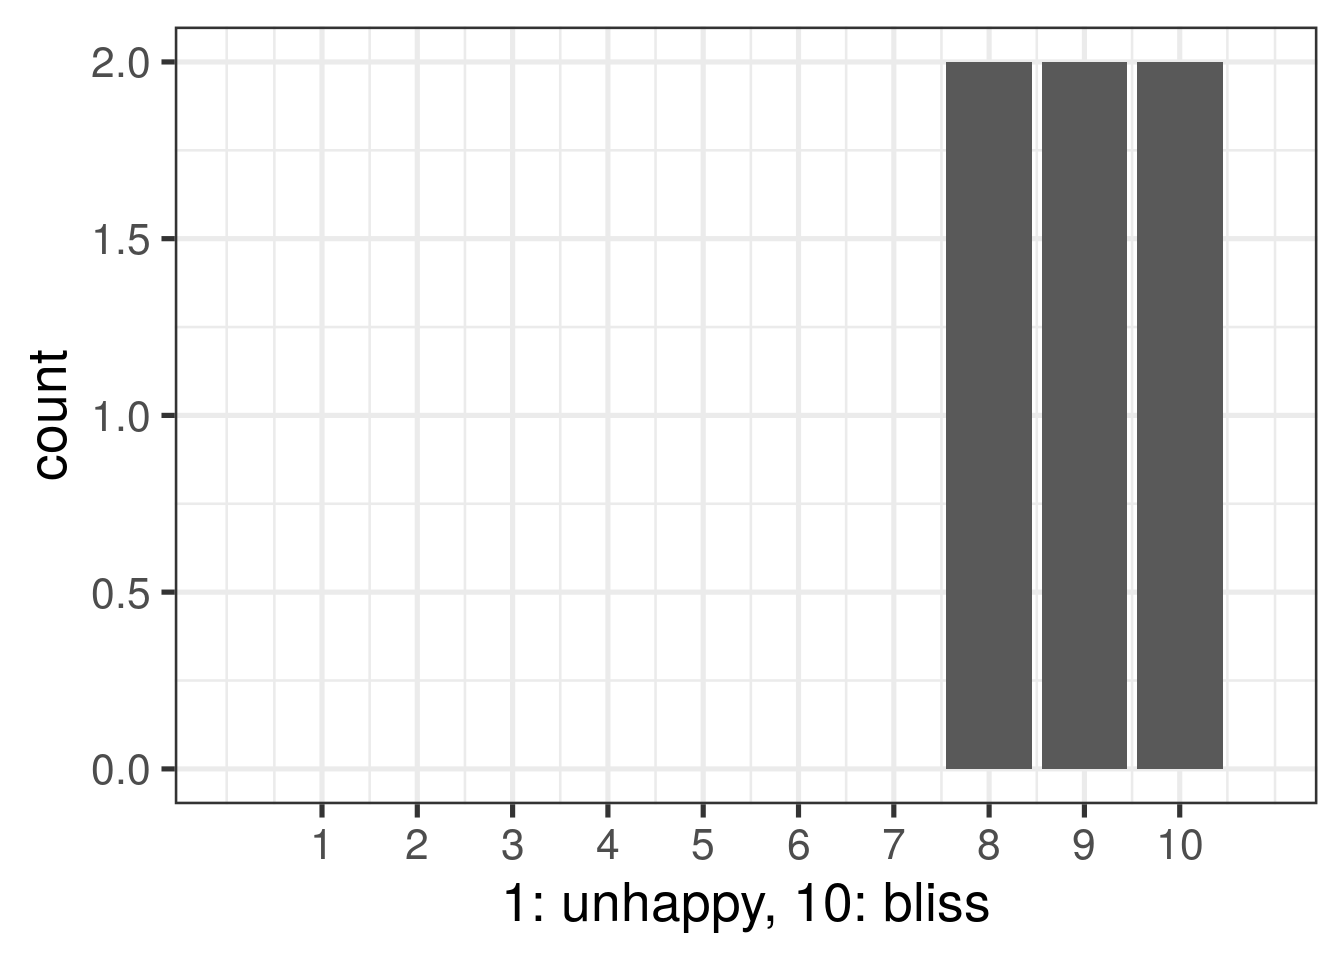
\includegraphics{_main_files/figure-latex/plot_5-1.pdf}

\hypertarget{is-there-something-that-could-be-provided-to-make-you-happier}{%
\section{Is there something that could be provided to make you happier?}\label{is-there-something-that-could-be-provided-to-make-you-happier}}

\begin{itemize}
\tightlist
\item
  upward career path.
\item
  Weighted blankets
\item
  Excited to get back in the lab and work more closely with others
\item
  I like working on projects with one other person
\item
  No.
\item
  No
\end{itemize}

\hypertarget{what-is-your-impression-of-social-life-in-the-team-too-social-not-enough-or-just-right-if-you-want-to-improve-the-social-life-in-the-lab-what-are-your-suggestions-for-achieving-this}{%
\section{What is your impression of social life in the team? Too social, not enough, or just right? If you want to improve the social life in the lab, what are your suggestions for achieving this?}\label{what-is-your-impression-of-social-life-in-the-team-too-social-not-enough-or-just-right-if-you-want-to-improve-the-social-life-in-the-lab-what-are-your-suggestions-for-achieving-this}}

\begin{itemize}
\tightlist
\item
  Social life is right
\item
  Hard to answer this question given that we've been WFH for over a year - I think we are the right amount of social
\item
  It feels not quite social enough, but this probably mostly has to do with inherent COVID restrictions which can't be easily avoided. I'm not sure the best way to improve.
\item
  I think we are doing what we can with the extenuating circumstances. I am glad we are getting back to doing happy hours now the weather is nice.
\item
  once the pandemic is closer i think the team will get to know each other better.
\item
  I think we could be a bit more social, but it's difficult right now during the pandemic
\end{itemize}

\hypertarget{how-comfortable-do-you-feel-sharing-personal-concerns-housing-financial-family-physical-or-mental-health-with-me}{%
\section{How comfortable do you feel sharing personal concerns (housing, financial, family, physical or mental health) with me?}\label{how-comfortable-do-you-feel-sharing-personal-concerns-housing-financial-family-physical-or-mental-health-with-me}}

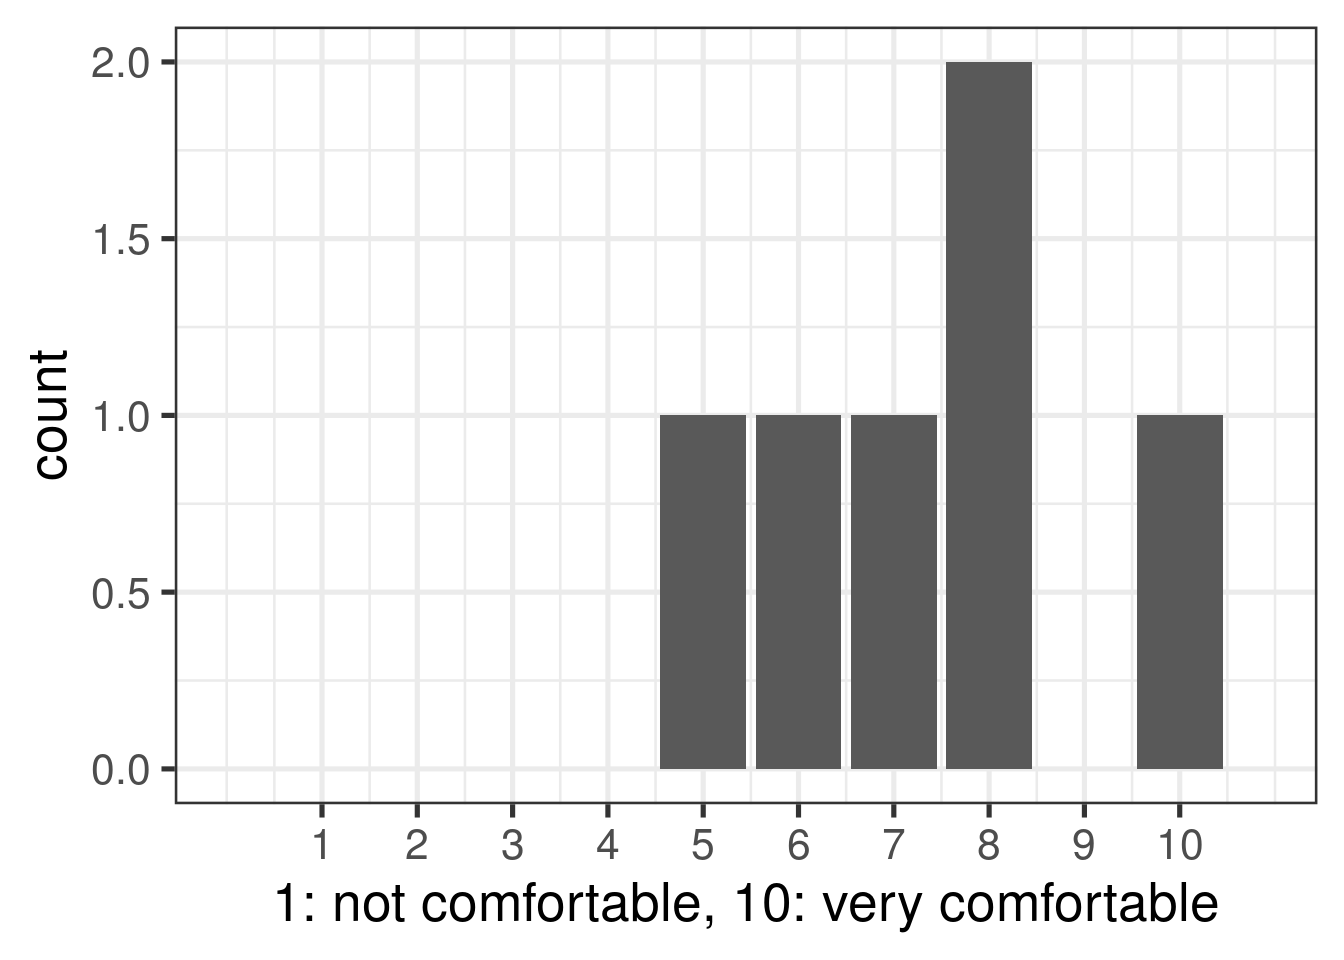
\includegraphics{_main_files/figure-latex/plot_8-1.pdf}

\hypertarget{do-you-feel-explicit-or-implicit-pressure-to-work-more-hours-than-you-feel-is-healthy}{%
\section{Do you feel explicit or implicit pressure to work more hours than you feel is healthy?}\label{do-you-feel-explicit-or-implicit-pressure-to-work-more-hours-than-you-feel-is-healthy}}

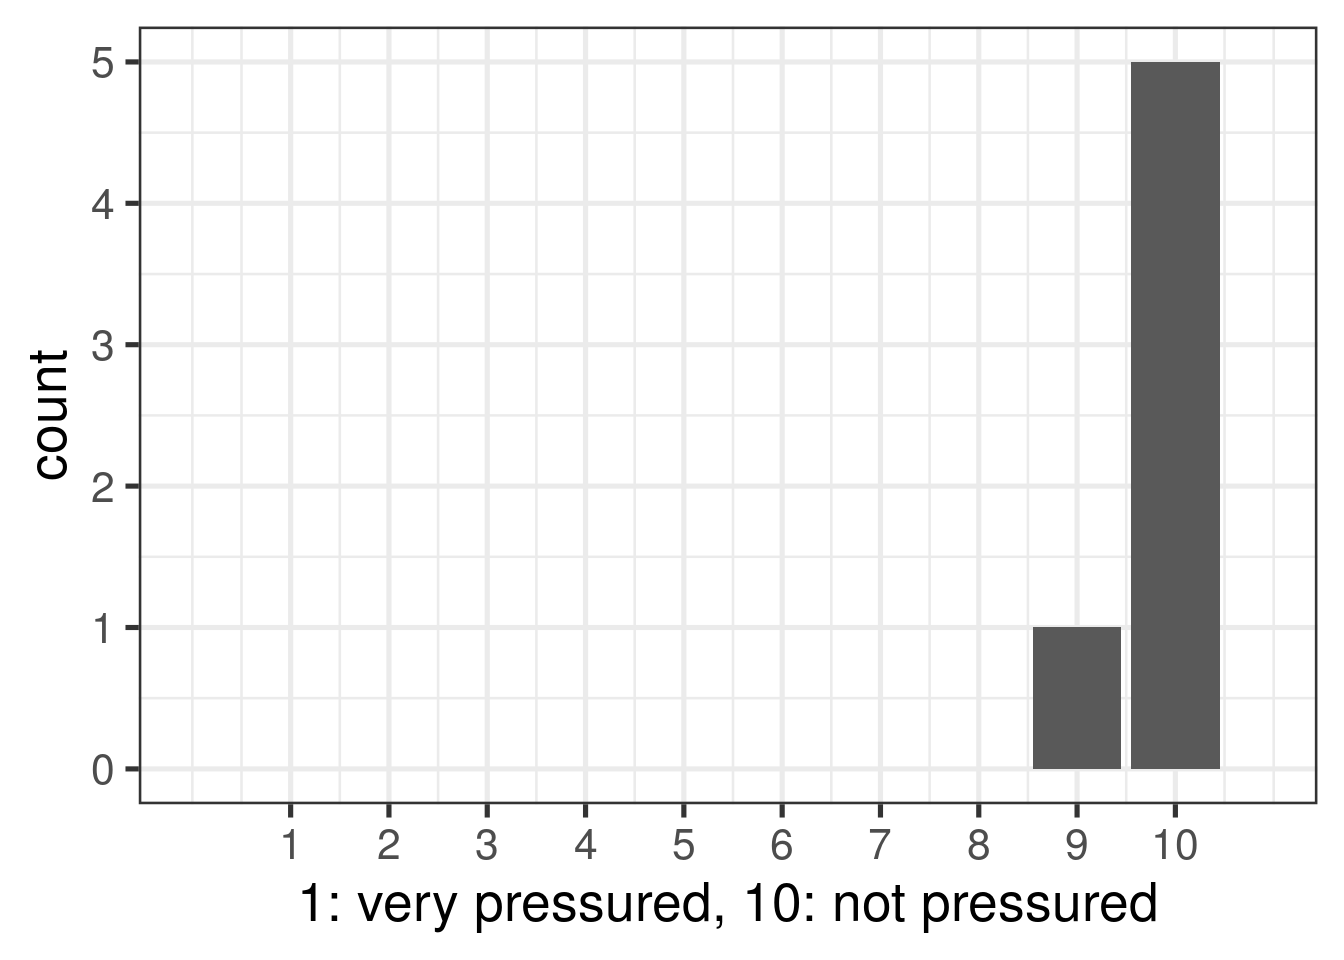
\includegraphics{_main_files/figure-latex/plot_9-1.pdf}

\hypertarget{do-you-feel-explicit-or-implicit-pressure-to-avoid-taking-vacations}{%
\section{Do you feel explicit or implicit pressure to avoid taking vacations?}\label{do-you-feel-explicit-or-implicit-pressure-to-avoid-taking-vacations}}

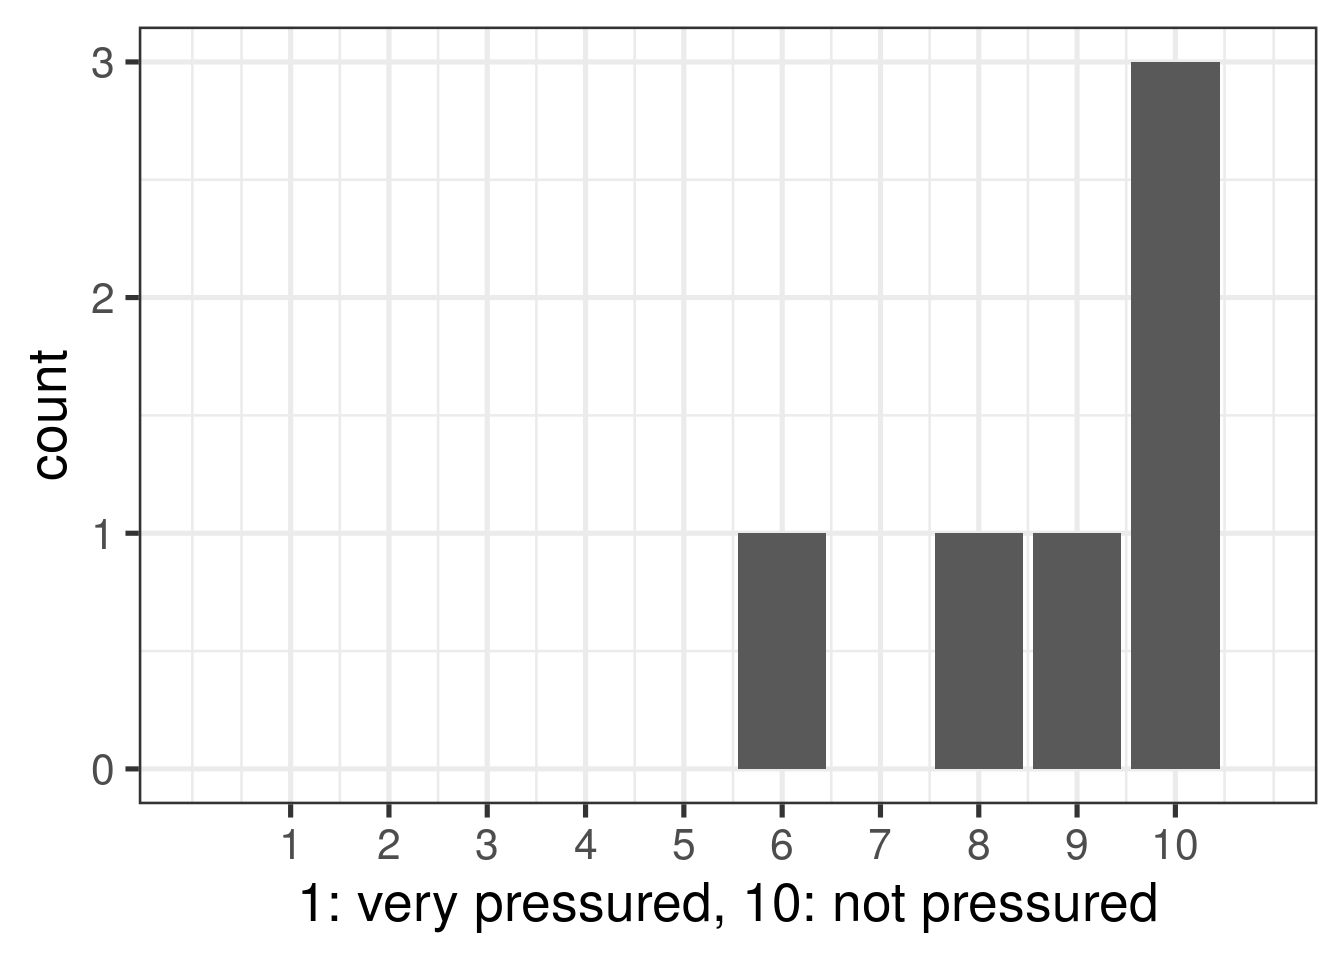
\includegraphics{_main_files/figure-latex/plot_10-1.pdf}

\hypertarget{have-you-experienced-or-witnessed-a-hostile-work-environment-in-the-team-bullying-gender-harassment-sexual-harassment}{%
\section{Have you experienced or witnessed a hostile work environment in the team? (bullying, gender harassment, sexual harassment)}\label{have-you-experienced-or-witnessed-a-hostile-work-environment-in-the-team-bullying-gender-harassment-sexual-harassment}}

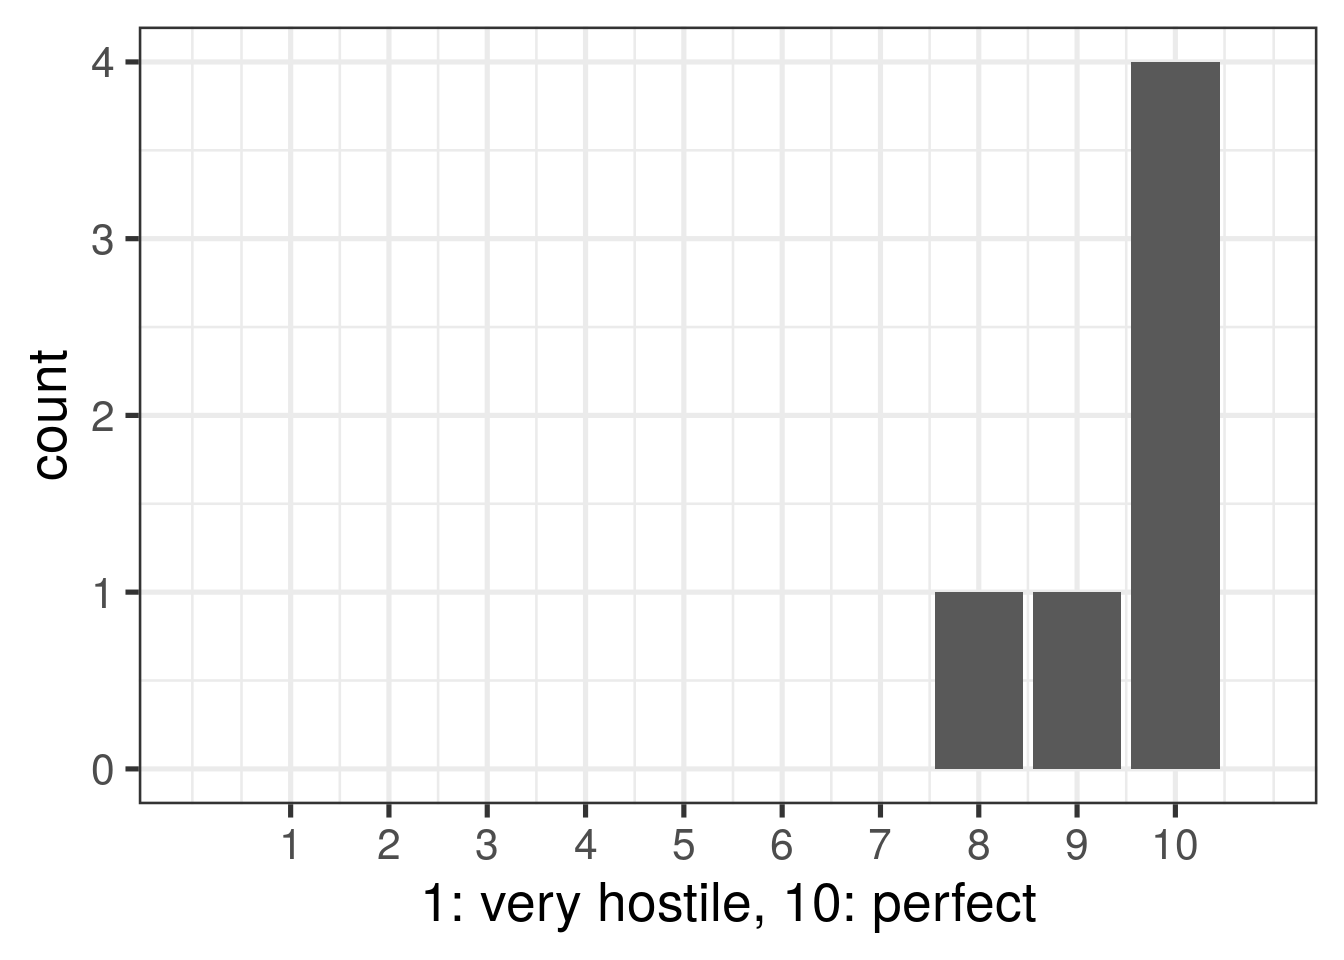
\includegraphics{_main_files/figure-latex/plot_11-1.pdf}

\hypertarget{how-well-does-the-team-communicate-as-a-whole}{%
\section{How well does the team communicate as a whole?}\label{how-well-does-the-team-communicate-as-a-whole}}

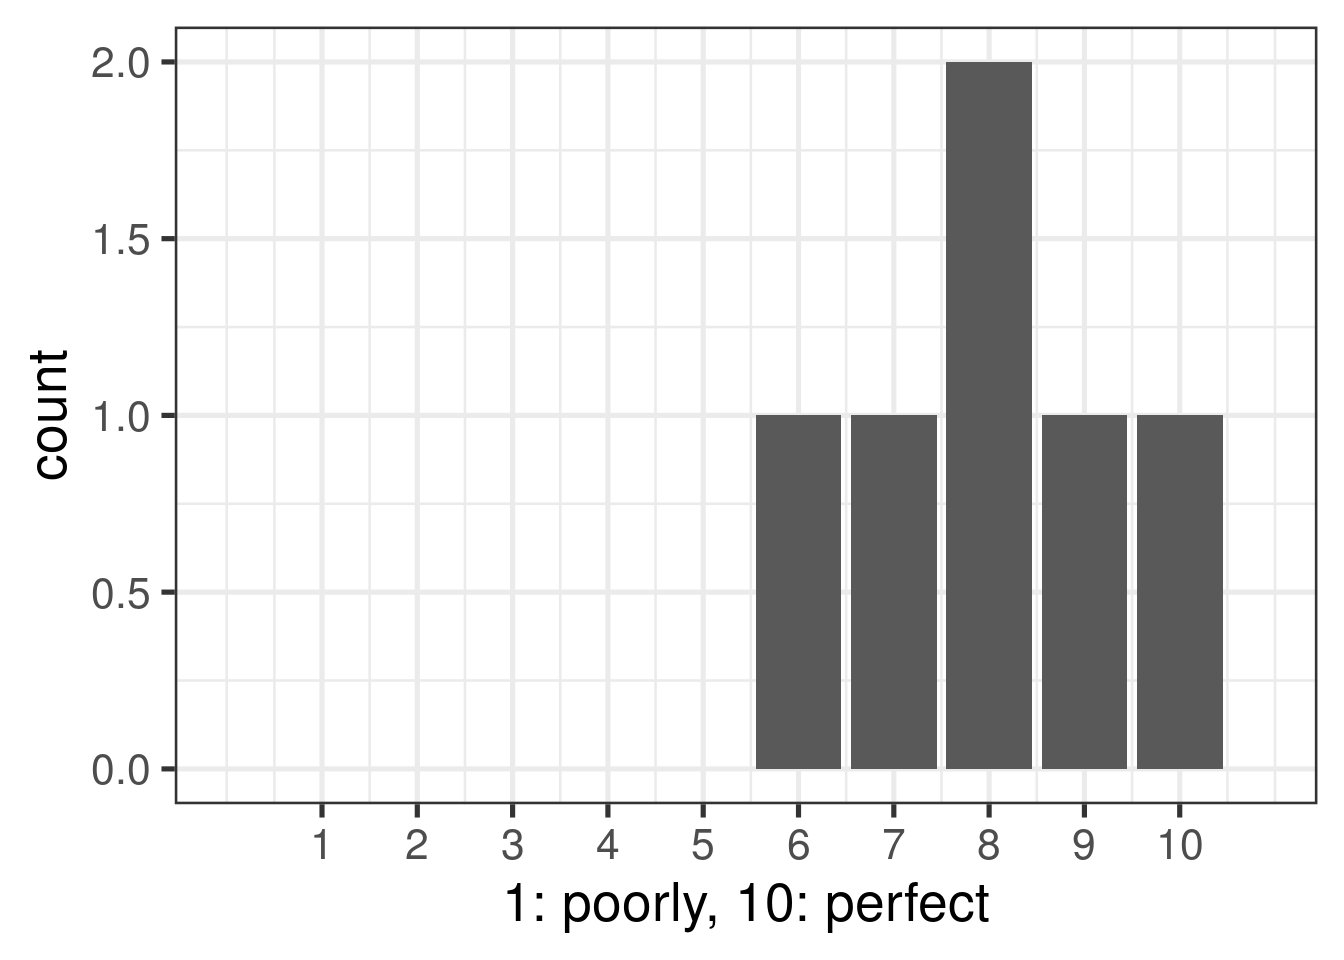
\includegraphics{_main_files/figure-latex/plot_12-1.pdf}

\hypertarget{what-are-some-ways-that-we-could-improve-communication-in-the-team}{%
\section{What are some ways that we could improve communication in the team?}\label{what-are-some-ways-that-we-could-improve-communication-in-the-team}}

\begin{itemize}
\tightlist
\item
  I liked discussing the ``nuts and bolts'' of our cluster usage/needs. Maybe we can focus some of our lab discussions on the tech/code side in addition to the science side. Also we never really put together the code review sessions and I feel like that would be a useful tool. Some times I am unsure which meetings I am expected to attend.
\item
  On personal projects, it's sometimes hard to get as much external feedback as would be ideal. Assigning multiple people to a particular project can improve internal communication and reduce the need for frequent feedback from you.
\item
  I think it is ok and slack is a perfect platform to do it.
\item
  We need to encourage more collaboration to develop less experienced members as well as encourage people to ask for help faster.
\item
  I feel like whatever answer I would give to this question is less relevant now that Lieber is opening back up
\item
  I think that we communicate very well.
\end{itemize}

\hypertarget{do-you-feel-that-lab-rulespolicies-are-clear-are-there-unspoken-rules-or-policies-that-you-feel-should-be-more-clearly-communicated}{%
\section{Do you feel that lab rules/policies are clear? Are there unspoken rules or policies that you feel should be more clearly communicated?}\label{do-you-feel-that-lab-rulespolicies-are-clear-are-there-unspoken-rules-or-policies-that-you-feel-should-be-more-clearly-communicated}}

\begin{itemize}
\tightlist
\item
  Rules are clear.
\item
  I feel pretty good about policies
\item
  if I had to give one, I would say baseline expectations across all projects
\item
  Rules are clear.
\item
  Lab rules are clear to me
\item
  I guess most rules are unspoken. I don't think we have a behavioral issue but any specific policies could be put in writing.
\end{itemize}

\hypertarget{are-there-policies-you-feel-should-be-explicitly-written-if-so-please-explain-which-ones.}{%
\section{Are there policies you feel should be explicitly written? If so, please explain which ones.}\label{are-there-policies-you-feel-should-be-explicitly-written-if-so-please-explain-which-ones.}}

\begin{itemize}
\tightlist
\item
  Guidelines for data privacy, what should we be careful to keep secure?
\item
  No
\item
  NA
\item
  No
\item
  No
\item
  No.
\end{itemize}

\hypertarget{do-you-feel-that-the-same-rules-apply-to-everyone-in-team-if-not-please-explain.}{%
\section{Do you feel that the same rules apply to everyone in team? If not, please explain.}\label{do-you-feel-that-the-same-rules-apply-to-everyone-in-team-if-not-please-explain.}}

\begin{itemize}
\item
  Yes
\item
  \begin{itemize}
  \tightlist
  \item
  \end{itemize}
\item
  Yes
\item
  Yes.
\item
  Yes
\item
  yes
\end{itemize}

\hypertarget{do-you-feel-empowered-to-make-suggestions-to-me-to-improve-the-team-culture-organization}{%
\section{Do you feel empowered to make suggestions to me to improve the team culture/ organization?}\label{do-you-feel-empowered-to-make-suggestions-to-me-to-improve-the-team-culture-organization}}

\begin{itemize}
\tightlist
\item
  Yes
\item
  Yes
\item
  Yes
\item
  Yes
\item
  Yes
\item
  Yes
\end{itemize}

\hypertarget{do-you-feel-empowered-to-make-suggestions-to-your-colleagues-to-improve-the-team-culture-organization}{%
\section{Do you feel empowered to make suggestions to your colleagues to improve the team culture/ organization?}\label{do-you-feel-empowered-to-make-suggestions-to-your-colleagues-to-improve-the-team-culture-organization}}

\begin{itemize}
\tightlist
\item
  Yes
\item
  Yes
\item
  Yes
\item
  Yes
\item
  Yes
\item
  Yes
\end{itemize}

\hypertarget{if-you-do-not-feel-empowered-to-make-suggestions-to-your-colleagues-in-the-team-or-to-me-to-improve-the-team-culture-organization-please-tell-me-more-about-this.}{%
\section{If you do not feel empowered to make suggestions to your colleagues in the team or to me to improve the team culture/ organization, please tell me more about this.}\label{if-you-do-not-feel-empowered-to-make-suggestions-to-your-colleagues-in-the-team-or-to-me-to-improve-the-team-culture-organization-please-tell-me-more-about-this.}}

\begin{itemize}
\item
  N/A
\item
  NA
\item
  NA
\item
  NA
\item
  \begin{itemize}
  \tightlist
  \item
  \end{itemize}
\item
  N/A
\end{itemize}

\hypertarget{do-you-feel-you-have-enough-feedback-on-your-project}{%
\section{Do you feel you have enough feedback on your project?}\label{do-you-feel-you-have-enough-feedback-on-your-project}}

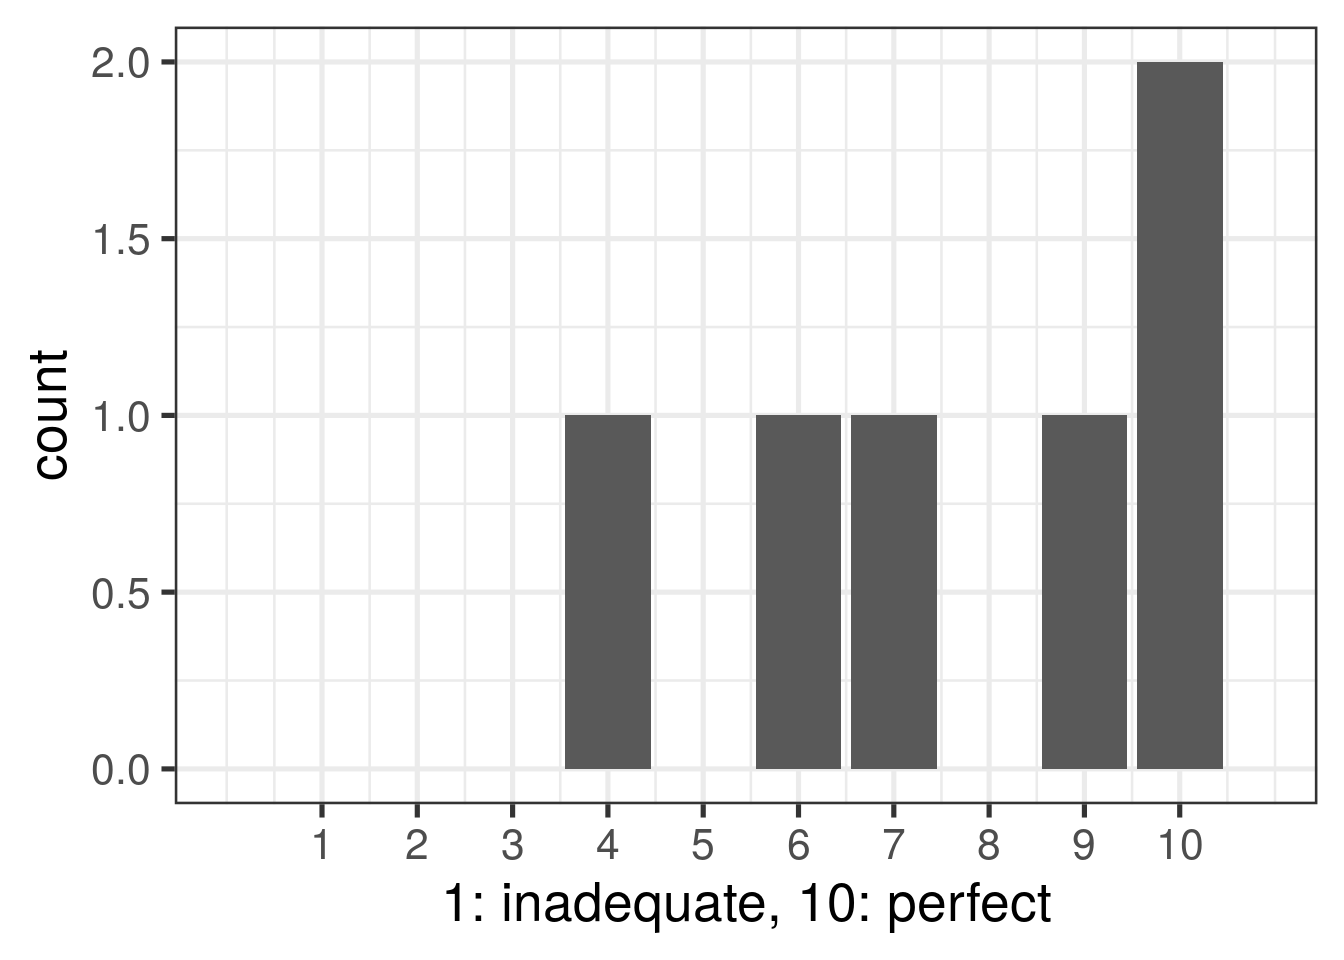
\includegraphics{_main_files/figure-latex/plot_20-1.pdf}

\hypertarget{do-you-feel-you-have-enough-time-to-meet-with-me}{%
\section{Do you feel you have enough time to meet with me?}\label{do-you-feel-you-have-enough-time-to-meet-with-me}}

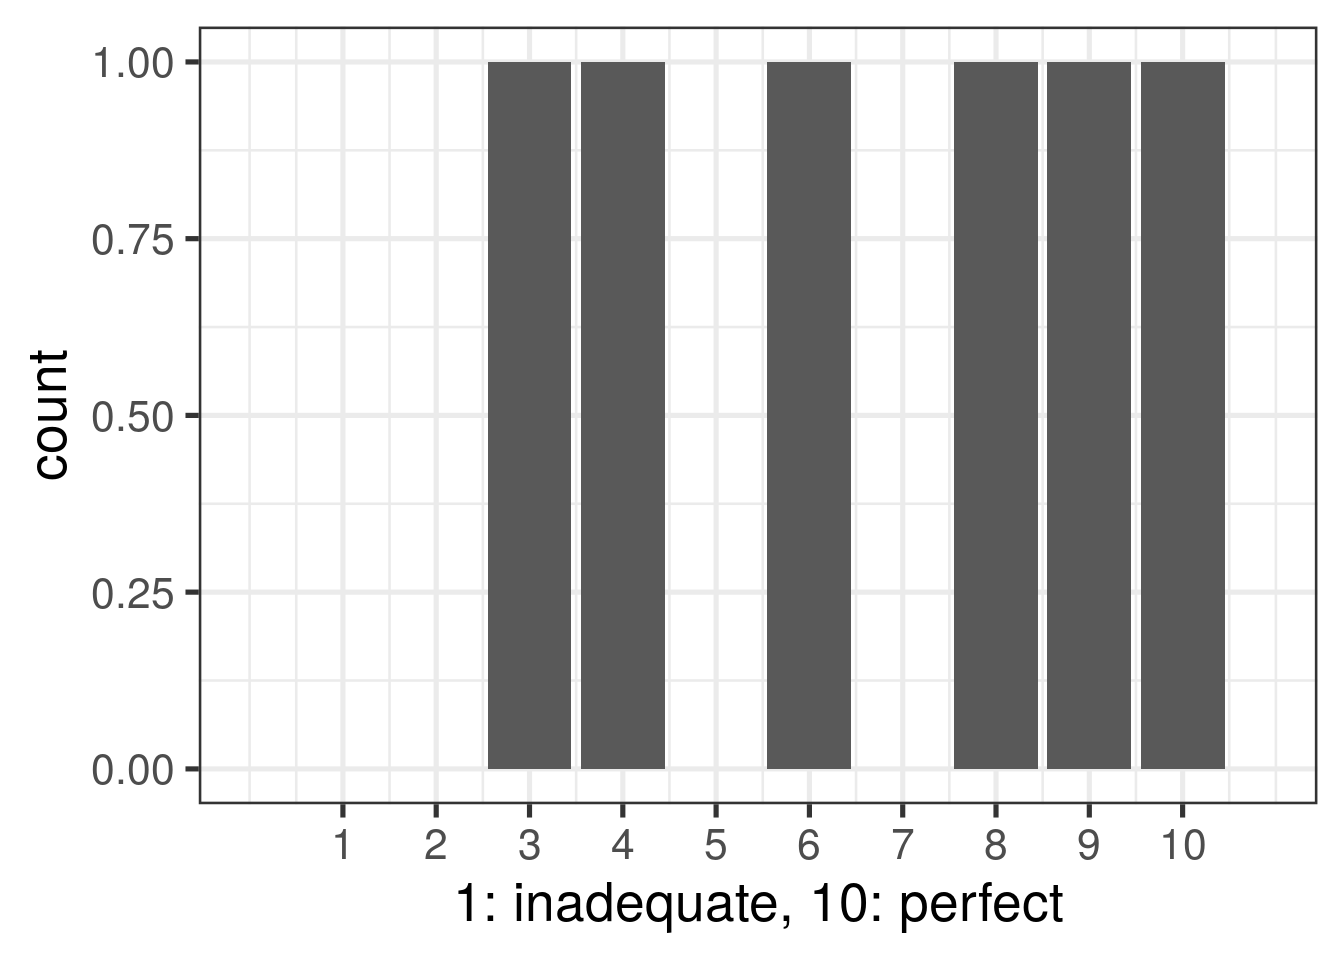
\includegraphics{_main_files/figure-latex/plot_21-1.pdf}

\hypertarget{how-useful-do-you-find-one-on-one-meetings-with-me}{%
\section{How useful do you find one-on-one meetings with me?}\label{how-useful-do-you-find-one-on-one-meetings-with-me}}

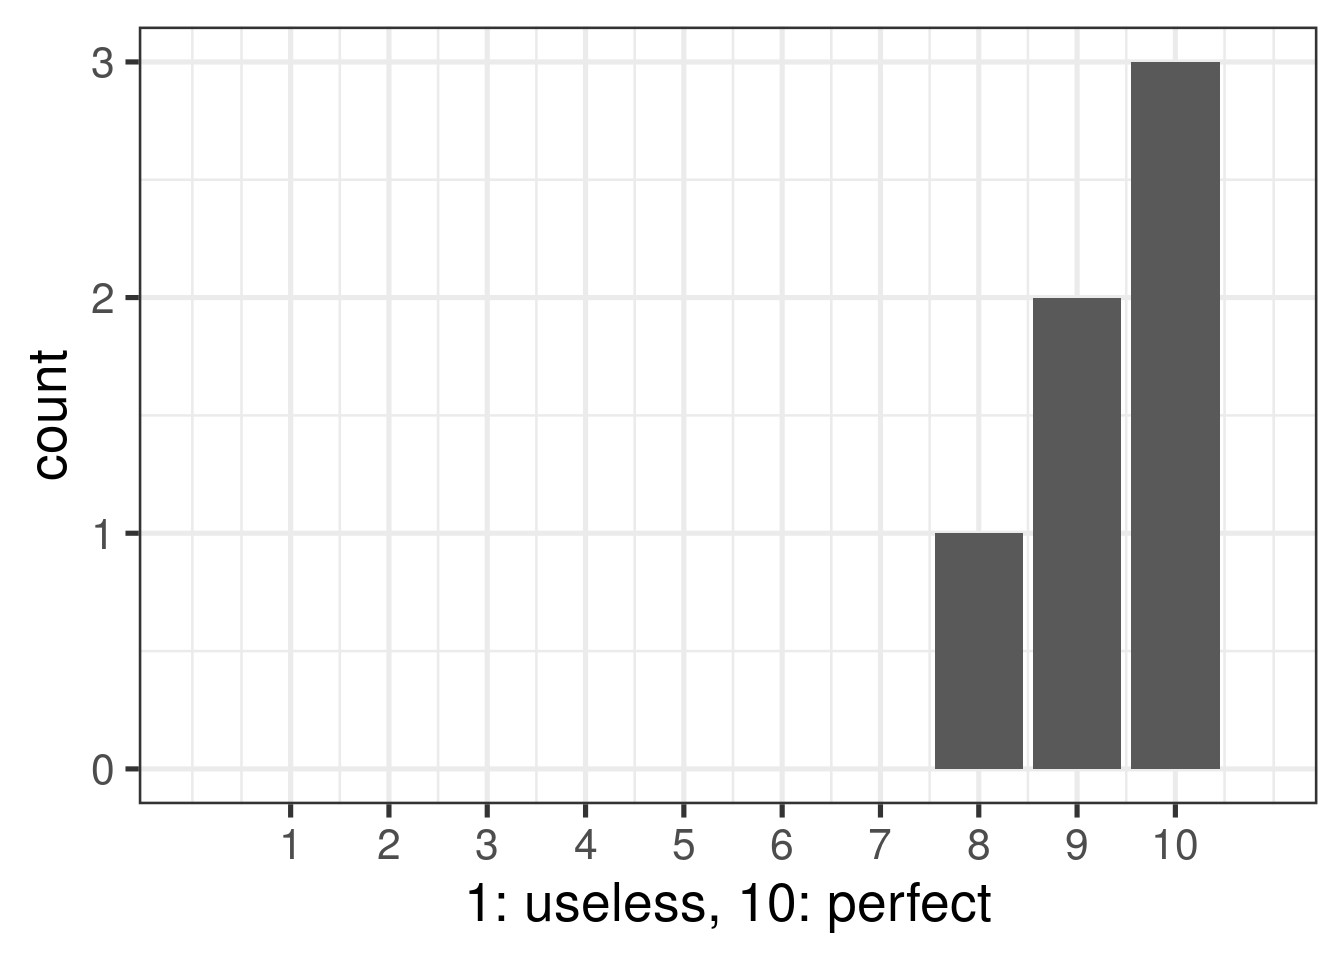
\includegraphics{_main_files/figure-latex/plot_22-1.pdf}

\hypertarget{is-there-something-that-could-make-these-meetings-more-useful-or-productive}{%
\section{Is there something that could make these meetings more useful or productive?}\label{is-there-something-that-could-make-these-meetings-more-useful-or-productive}}

\begin{itemize}
\tightlist
\item
  No, they are productive.
\item
  NA
\item
  My meetings with you are always very helpful.
\item
  I think the 1on1s on Monday could be a bit longer, sometimes it feels rushed and I feel bad delaying the next meeting if I have a few more things to say. I preferred having a longer and more flexible 1on1 built in to the week.
\item
  Maybe an agenda
\item
  I think everything is okay
\end{itemize}

\hypertarget{do-you-think-the-current-system-of-formal-scheduled-weekly-one-on-one-meetings-is-working-should-these-be-less-frequent-more-frequent-or-stay-as-is}{%
\section{Do you think the current system of formal scheduled weekly one-on-one meetings is working? Should these be less frequent, more frequent, or stay as is?}\label{do-you-think-the-current-system-of-formal-scheduled-weekly-one-on-one-meetings-is-working-should-these-be-less-frequent-more-frequent-or-stay-as-is}}

\begin{itemize}
\tightlist
\item
  I think once a week is a good frequency
\item
  As is is fine, might like more time but I could request it on Calendly
\item
  The current system is good.
\item
  Yes and maybe paired analysis sessions would be good
\item
  I think weekly is good.
\item
  It works and I really like this system. I think it should stay as it is.
\end{itemize}

\hypertarget{do-you-think-you-would-benefit-from-more-formal-feedback-on-your-progress}{%
\section{Do you think you would benefit from more formal feedback on your progress?}\label{do-you-think-you-would-benefit-from-more-formal-feedback-on-your-progress}}

\begin{itemize}
\tightlist
\item
  I think the feedback I receive is excellent
\item
  Yes
\item
  Yes
\item
  Yes, especially when it comes to code in things I am learning
\item
  Yes, if possible, though it doesn't need to be formal.
\item
  No
\end{itemize}

\hypertarget{how-supported-do-you-feel-by-me-and-do-you-think-that-you-are-getting-the-mentoring-career-advice-and-general-guidance-to-succeed}{%
\section{How supported do you feel by me, and do you think that you are getting the mentoring, career advice, and general guidance to succeed?}\label{how-supported-do-you-feel-by-me-and-do-you-think-that-you-are-getting-the-mentoring-career-advice-and-general-guidance-to-succeed}}

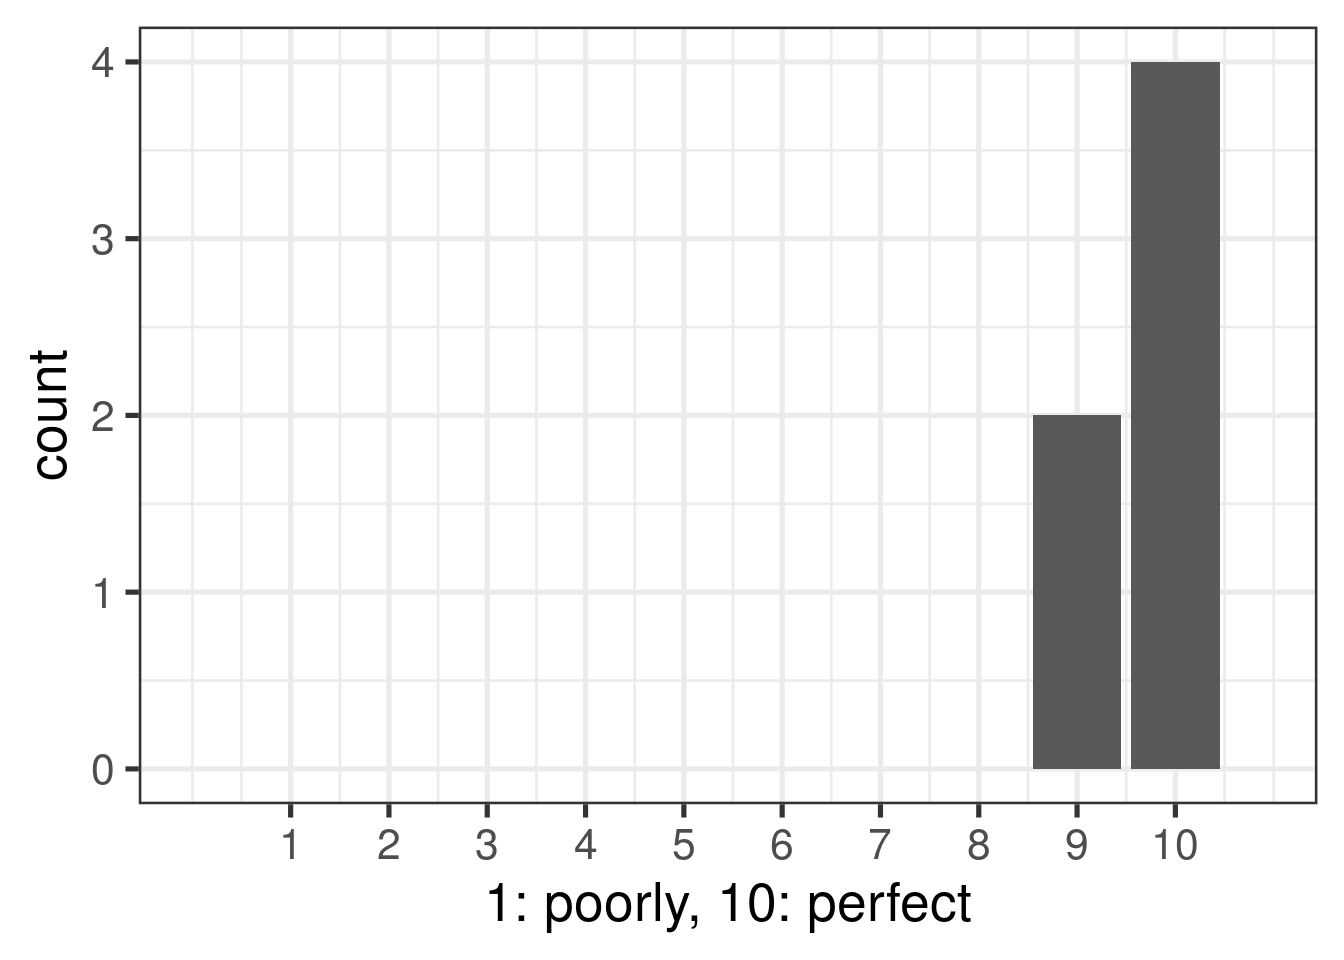
\includegraphics{_main_files/figure-latex/plot_26-1.pdf}

\hypertarget{do-you-want-formal-training-in-giving-talks}{%
\section{Do you want formal training in giving talks?}\label{do-you-want-formal-training-in-giving-talks}}

\begin{itemize}
\tightlist
\item
  Yes
\item
  Yes
\item
  Yes
\item
  Yes
\item
  No
\item
  Yes
\end{itemize}

\hypertarget{do-you-want-to-have-an-annual-mentoring-meeting-to-go-over-your-individual-development-plan-and-discuss-post-phd-or-post-postdoc-plans-leo-edit-see-httpslcolladotor.github.iobioc_team_dscareer-growth.html.}{%
\section{\texorpdfstring{Do you want to have an Annual Mentoring Meeting to go over your Individual Development Plan and discuss post-PhD or post-Postdoc plans? Leo edit: see \url{https://lcolladotor.github.io/bioc_team_ds/career-growth.html}.}{Do you want to have an Annual Mentoring Meeting to go over your Individual Development Plan and discuss post-PhD or post-Postdoc plans? Leo edit: see https://lcolladotor.github.io/bioc\_team\_ds/career-growth.html.}}\label{do-you-want-to-have-an-annual-mentoring-meeting-to-go-over-your-individual-development-plan-and-discuss-post-phd-or-post-postdoc-plans-leo-edit-see-httpslcolladotor.github.iobioc_team_dscareer-growth.html.}}

\begin{itemize}
\tightlist
\item
  Yes
\item
  Yes
\item
  Yes
\item
  Yes
\item
  Yes
\item
  Yes
\end{itemize}

\hypertarget{what-kind-of-advice-or-information-would-be-useful-to-discuss-at-such-an-annual-mentoring-meeting}{%
\section{What kind of advice or information would be useful to discuss at such an Annual Mentoring Meeting?}\label{what-kind-of-advice-or-information-would-be-useful-to-discuss-at-such-an-annual-mentoring-meeting}}

\begin{itemize}
\tightlist
\item
  Career goals \& next steps at LIBD. Potential opportunities (projects, talks, ect.)
\item
  How to apply to phd programs. Leo and I have already talked about this.
\item
  How to get promoted
\item
  Our current annual meetings are formatted well.
\item
  Skills that need to be learned. Areas of weakness that need to be improved.
\item
  NA
\end{itemize}

\hypertarget{do-you-have-any-explicit-feedback-on-how-i-can-improve-my-mentoring-style}{%
\section{Do you have any explicit feedback on how I can improve my mentoring style?}\label{do-you-have-any-explicit-feedback-on-how-i-can-improve-my-mentoring-style}}

\begin{itemize}
\tightlist
\item
  Not really
\item
  Probably a little more structure in terms of expectations around progress and deadlines.
\item
  I think you're a great mentor.
\item
  No
\item
  The current style is very good.
\item
  NA
\end{itemize}

\hypertarget{do-you-feel-it-is-easy-to-get-information-from-me}{%
\section{Do you feel it is easy to get information from me?}\label{do-you-feel-it-is-easy-to-get-information-from-me}}

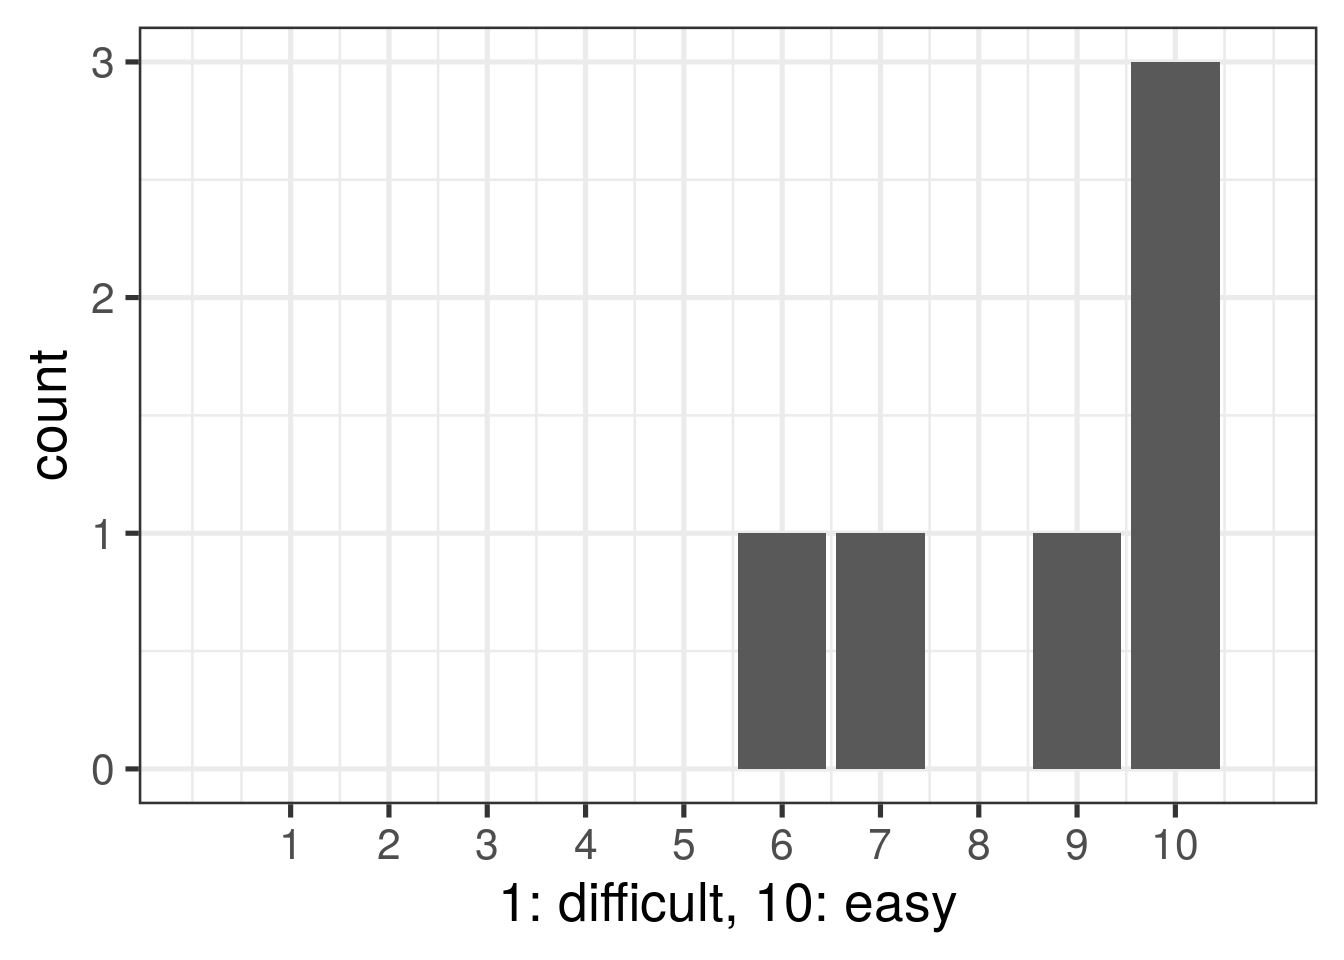
\includegraphics{_main_files/figure-latex/plot_31-1.pdf}

\hypertarget{do-you-feel-it-is-easy-to-get-information-from-other-people-in-the-team}{%
\section{Do you feel it is easy to get information from other people in the team?}\label{do-you-feel-it-is-easy-to-get-information-from-other-people-in-the-team}}

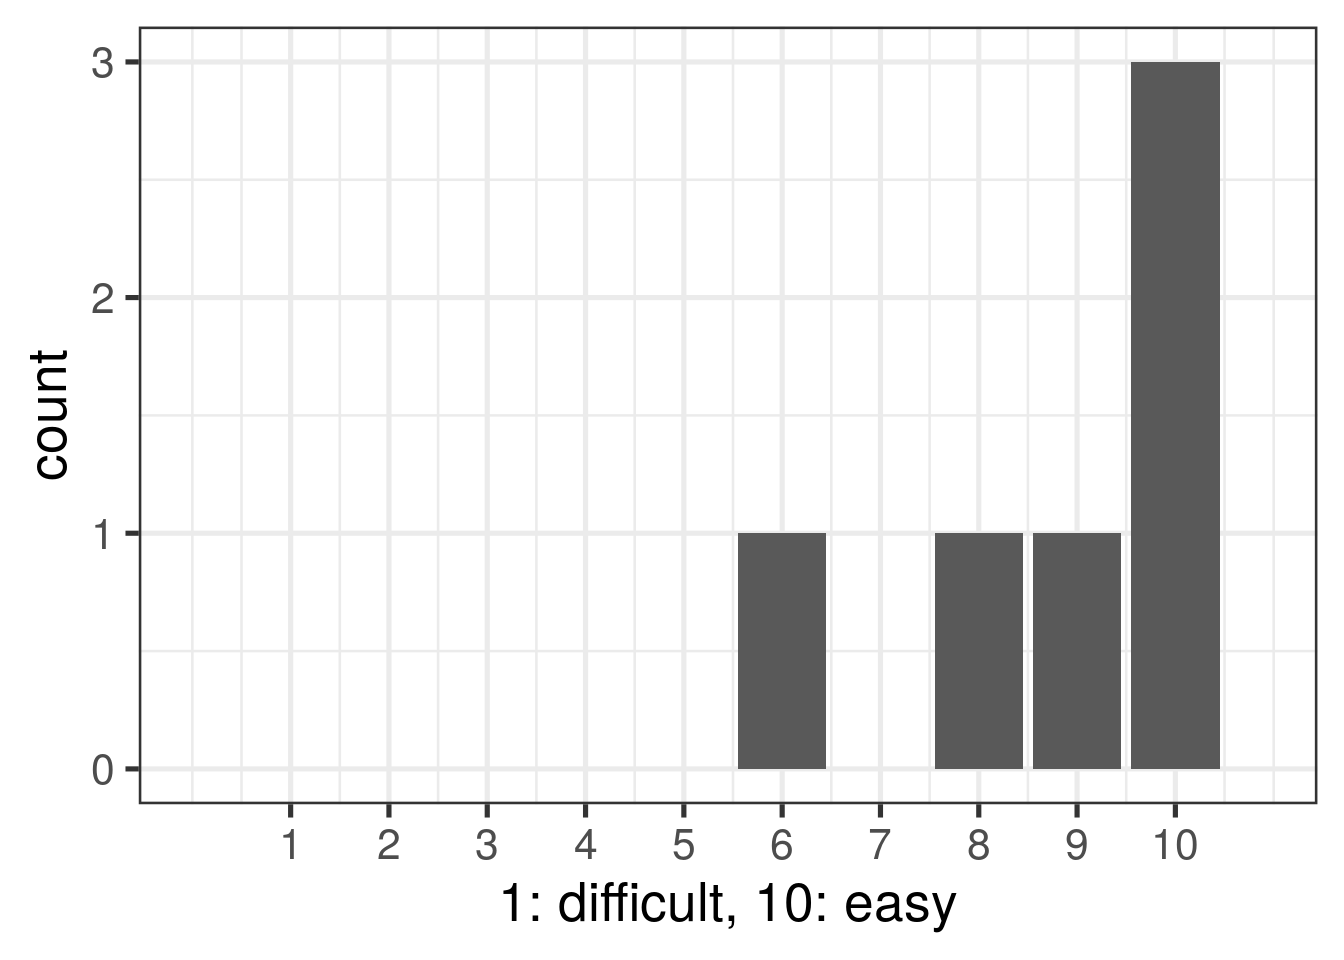
\includegraphics{_main_files/figure-latex/plot_32-1.pdf}

\hypertarget{how-useful-do-you-find-team-meetings}{%
\section{How useful do you find team meetings?}\label{how-useful-do-you-find-team-meetings}}

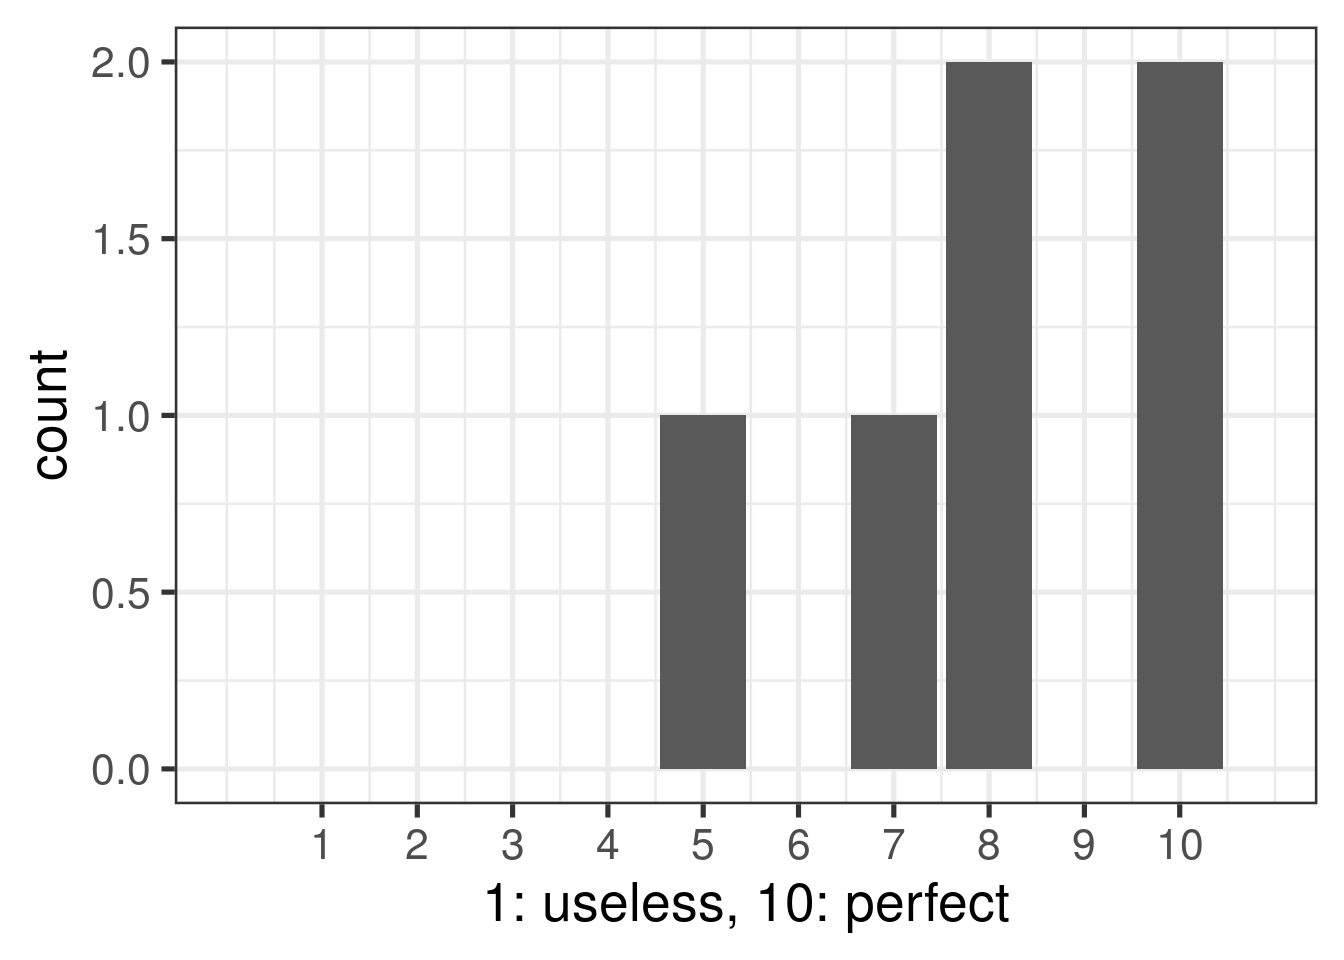
\includegraphics{_main_files/figure-latex/plot_33-1.pdf}

\hypertarget{is-there-something-that-could-make-team-meetings-more-useful-or-productive}{%
\section{Is there something that could make team meetings more useful or productive?}\label{is-there-something-that-could-make-team-meetings-more-useful-or-productive}}

\begin{itemize}
\tightlist
\item
  Maybe a scheduled agenda
\item
  they're more or less fine as-is. The only thing I can think of that could be useful is having someone take meeting notes, so we know what was covered. Not urgent though.
\item
  I think our meetings are very productive.
\item
  It's nice to hear what everyone is up to in their individual projects, but its not always useful (it can be easy to check out). Maybe we could make the Notion board more of a part of it? Do a number rundown (we put up x number of tasks to do and got y done). It can be easy to forget the Notion board since we don't really engage with it at meetings. My favorite part of the when everyone gets chatting about a subject work related or not.
\item
  We could maybe focus more on problems we encounter/ are working on during the week.
\item
  No
\end{itemize}

\hypertarget{how-useful-do-you-find-sub-group-meetings}{%
\section{How useful do you find sub-group meetings?}\label{how-useful-do-you-find-sub-group-meetings}}

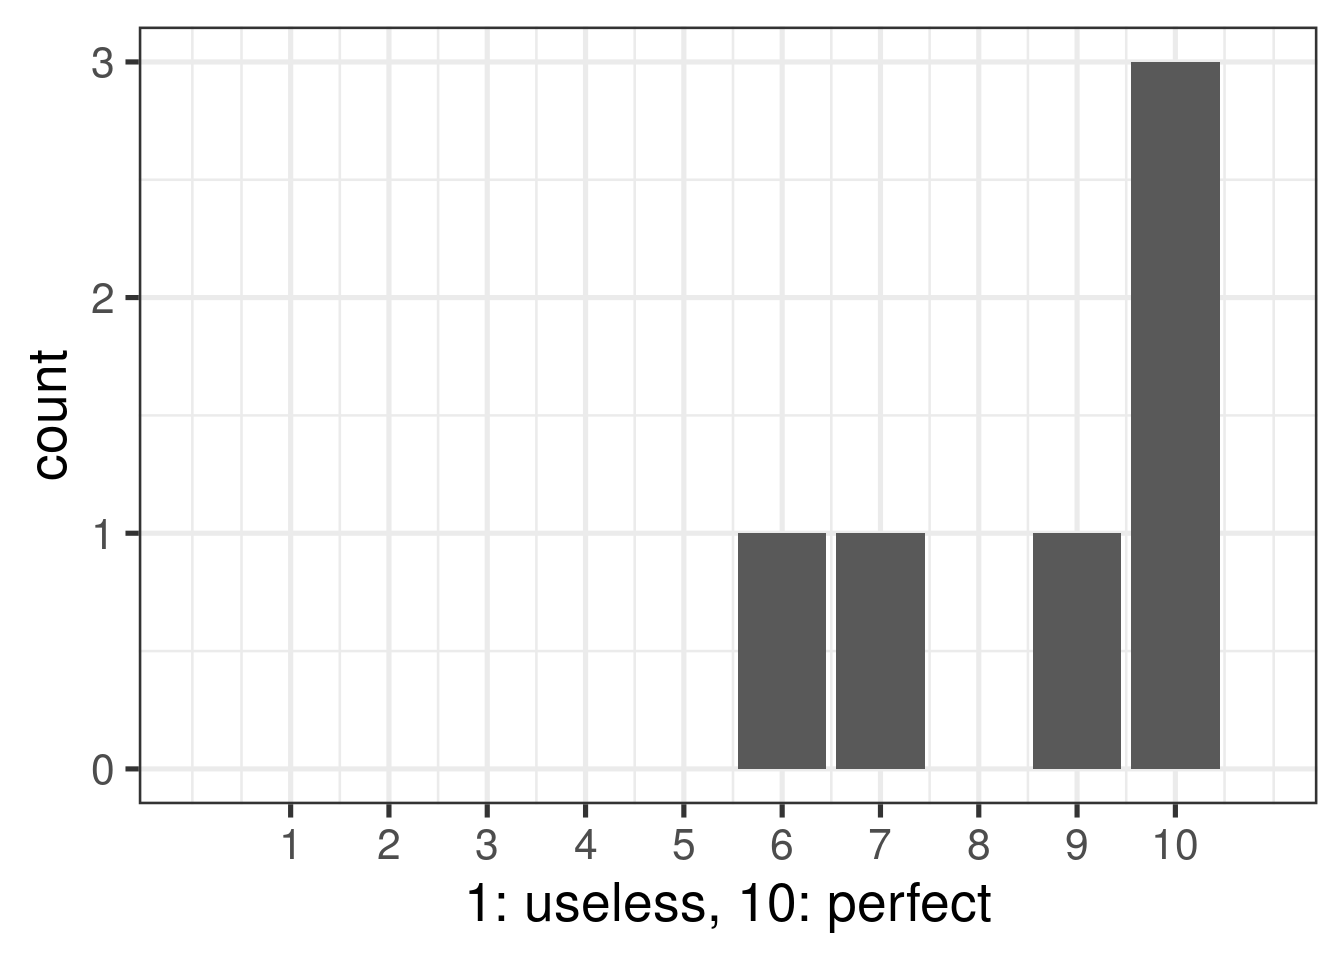
\includegraphics{_main_files/figure-latex/plot_35-1.pdf}

\hypertarget{is-there-something-that-could-make-sub-group-meetings-more-useful-or-productive}{%
\section{Is there something that could make sub-group meetings more useful or productive?}\label{is-there-something-that-could-make-sub-group-meetings-more-useful-or-productive}}

\begin{itemize}
\tightlist
\item
  N/A
\item
  No
\item
  I find meetings focused on one topic or goal to be the most productive, maybe make a conscious effort to record what progress/decisions were made on slack
\item
  No.
\item
  No
\item
  not entirely sure what a sub-group meeting is but if it's a meeting on a project or topic then I think they're fine as-is - maybe delegating note-taking would be and having a formal agenda after each meeting
\end{itemize}

\hypertarget{how-useful-do-you-find-the-journal-club}{%
\section{How useful do you find the journal club?}\label{how-useful-do-you-find-the-journal-club}}

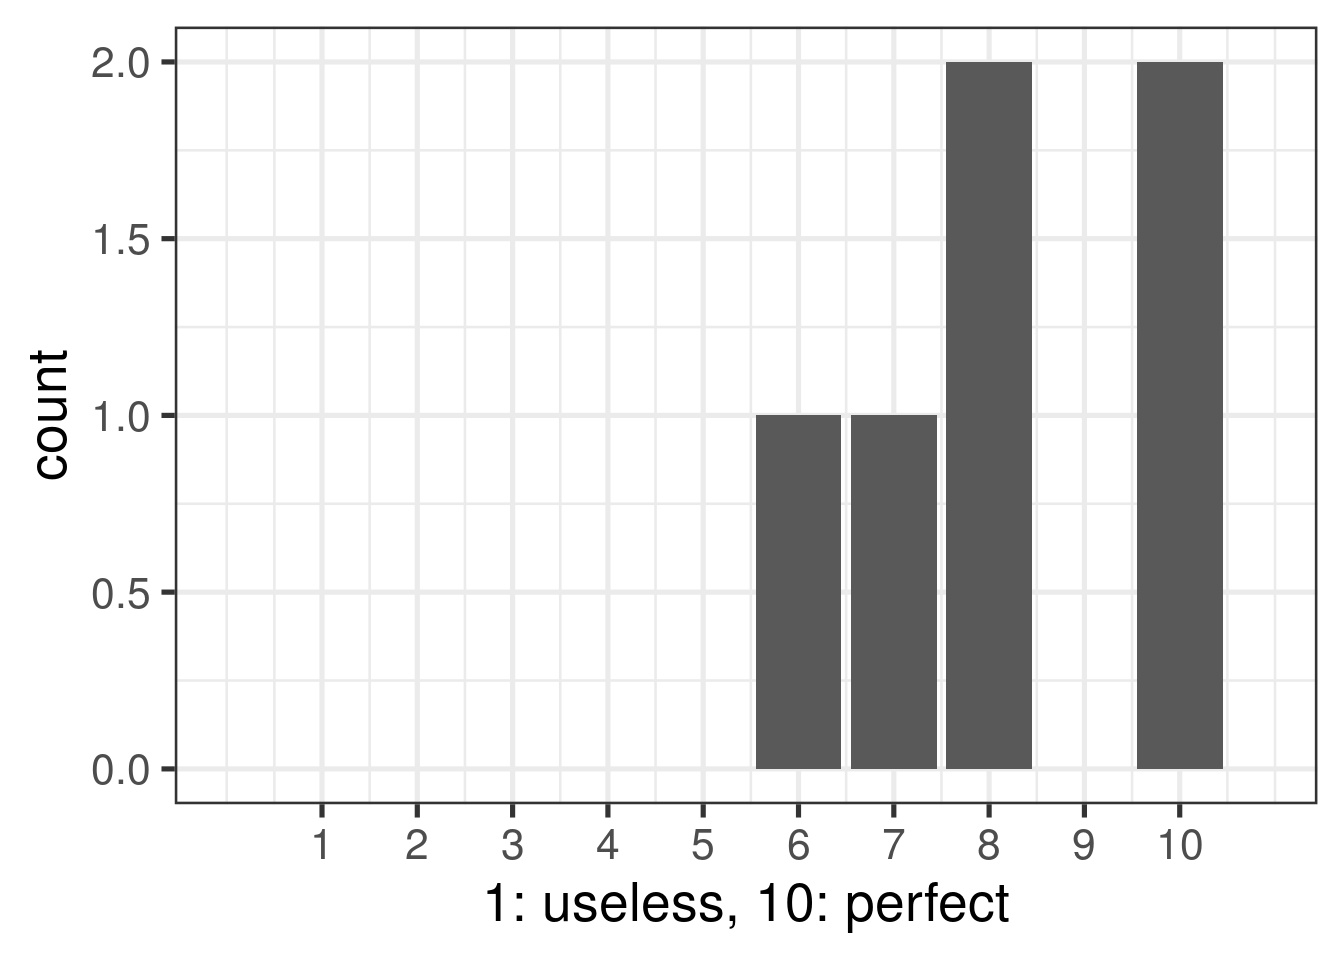
\includegraphics{_main_files/figure-latex/plot_37-1.pdf}

\hypertarget{is-there-something-that-could-make-the-journal-club-more-useful-or-productive}{%
\section{Is there something that could make the journal club more useful or productive?}\label{is-there-something-that-could-make-the-journal-club-more-useful-or-productive}}

\begin{itemize}
\tightlist
\item
  Sometimes journal club is on topics that are very far outside my realm of knowledge and the work I do. But that's ok because I get to learn about new things.
\item
  more accountability to read the article. I feel it's not as interactive as it could be.
\item
  some sort of shared repository for notes, or summary
\item
  No.
\item
  I find the journal club most useful when I am the one presenting because it forces me to learn a paper. If the paper someone else is presenting is too long or specific it can be hard to engage with it. Maybe more guidance on topics/how to find papers good for the club?
\item
  No
\end{itemize}

\hypertarget{how-much-freedom-do-you-feel-you-have-to-decide-how-you-do-your-work}{%
\section{How much freedom do you feel you have to decide how you do your work?}\label{how-much-freedom-do-you-feel-you-have-to-decide-how-you-do-your-work}}

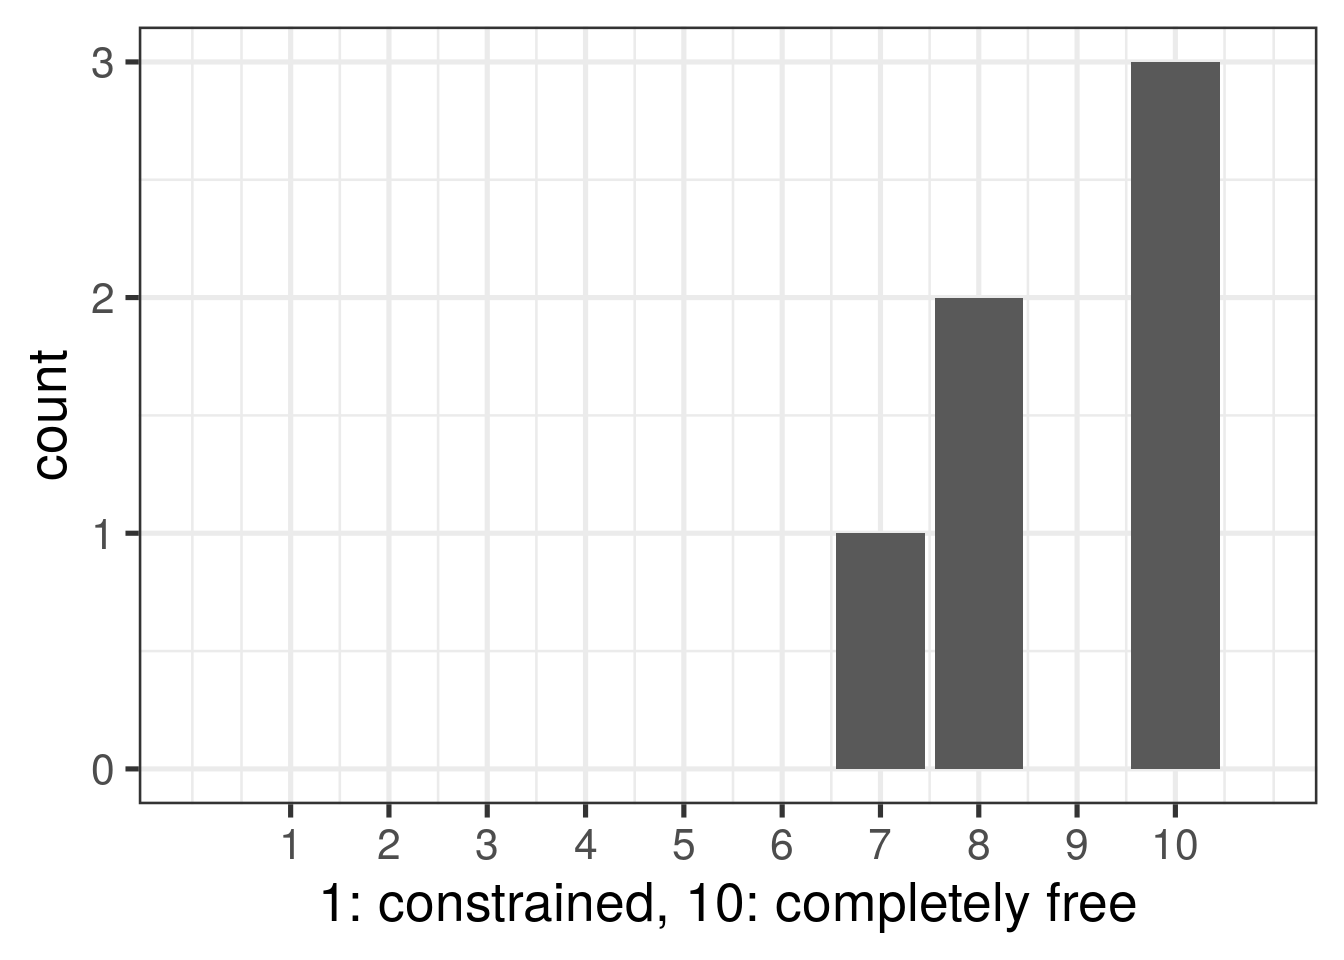
\includegraphics{_main_files/figure-latex/plot_39-1.pdf}

\hypertarget{how-collaborative-do-you-think-the-team-is}{%
\section{How collaborative do you think the team is?}\label{how-collaborative-do-you-think-the-team-is}}

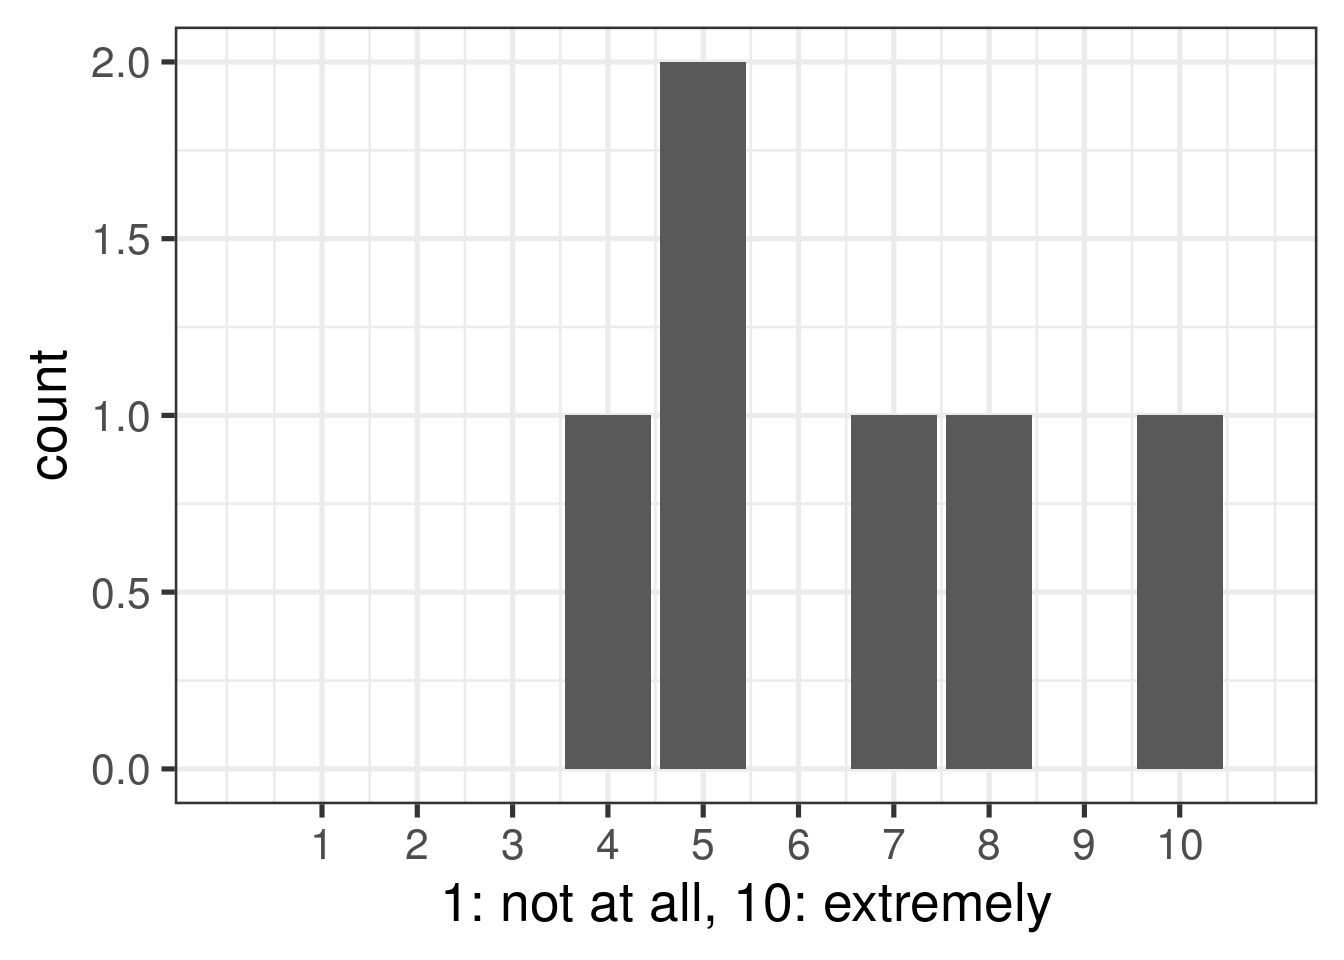
\includegraphics{_main_files/figure-latex/plot_40-1.pdf}

\hypertarget{do-you-perceive-that-there-is-any-favoritism-in-the-team-please-elaborate.}{%
\section{Do you perceive that there is any favoritism in the team? Please elaborate.}\label{do-you-perceive-that-there-is-any-favoritism-in-the-team-please-elaborate.}}

\begin{itemize}
\tightlist
\item
  No
\item
  no
\item
  No
\item
  No.
\item
  none whatsoever
\item
  No
\end{itemize}

\hypertarget{are-there-any-issues-with-collaborations-in-the-team-that-are-not-working-please-explain.}{%
\section{Are there any issues with collaborations in the team that are not working? Please explain.}\label{are-there-any-issues-with-collaborations-in-the-team-that-are-not-working-please-explain.}}

\begin{itemize}
\tightlist
\item
  No
\item
  No
\item
  No.
\item
  I feel good about the projects I am collaborating with others on
\item
  no
\item
  This has gotten better recently but I feel like collaborations do not happen all that often
\end{itemize}

\hypertarget{are-you-aware-of-the-teams-authorship-policies}{%
\section{Are you aware of the team's authorship policies?}\label{are-you-aware-of-the-teams-authorship-policies}}

\begin{itemize}
\tightlist
\item
  No
\item
  No
\item
  No
\item
  No
\item
  No
\item
  No
\end{itemize}

\hypertarget{do-have-any-concerns-about-anticipated-authorship-on-papers-describing-your-work-or-collaborations-that-you-are-involved-with}{%
\section{Do have any concerns about anticipated authorship on papers describing your work or collaborations that you are involved with?}\label{do-have-any-concerns-about-anticipated-authorship-on-papers-describing-your-work-or-collaborations-that-you-are-involved-with}}

\begin{itemize}
\tightlist
\item
  No
\item
  No
\item
  No
\item
  There needs to be upfront discussions with the labs we collaborate with about authorship
\item
  no
\item
  No, but authorship hasn't always been explicitly discussed.
\end{itemize}

\hypertarget{please-rate-whether-you-feel-the-team-provides-you-with-the-tools-and-technologies-you-need}{%
\section{Please rate whether you feel the team provides you with the tools and technologies you need?}\label{please-rate-whether-you-feel-the-team-provides-you-with-the-tools-and-technologies-you-need}}

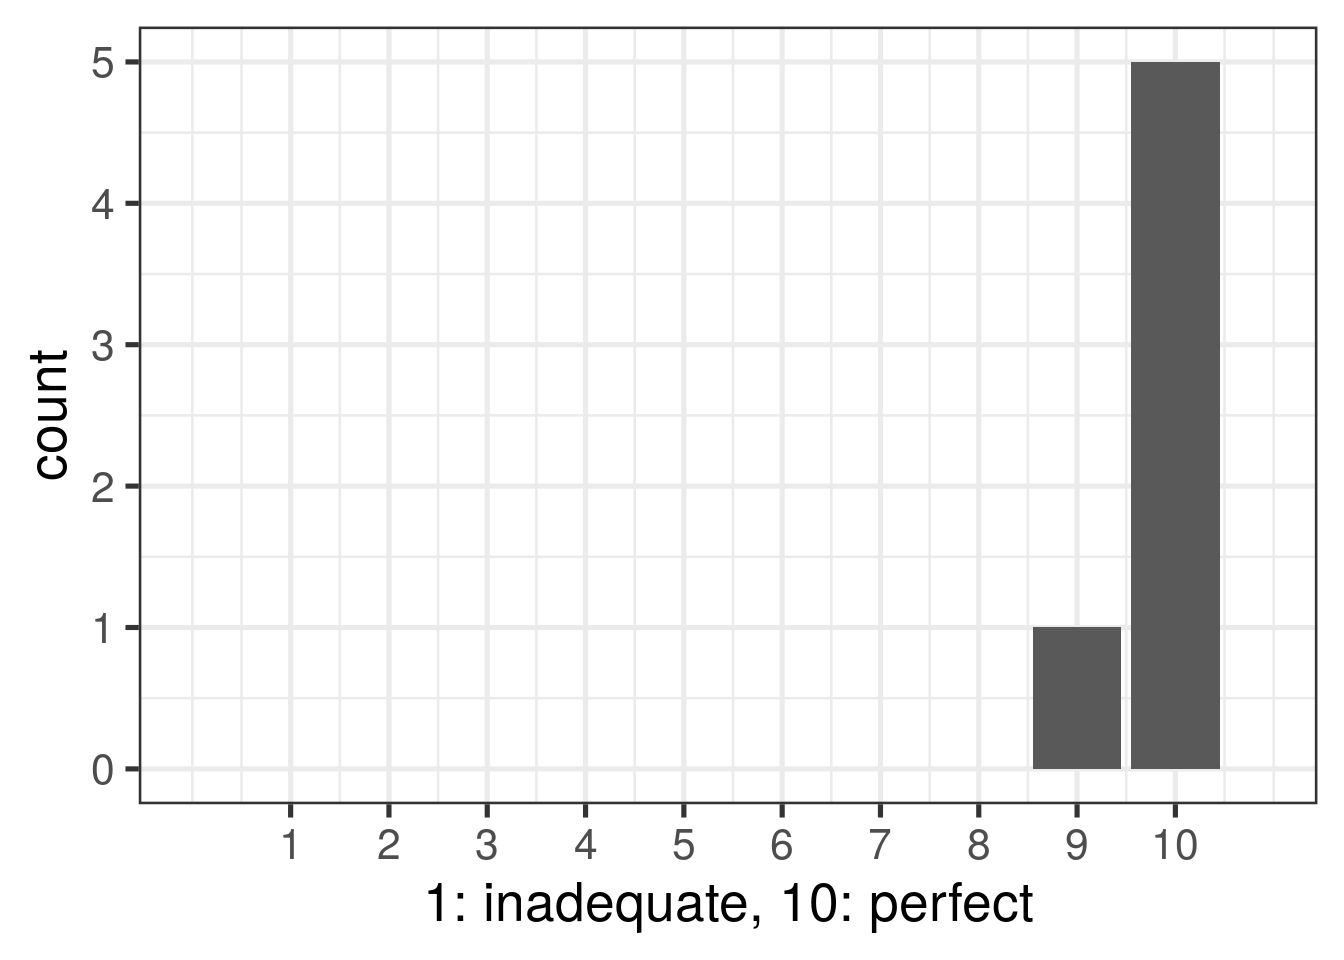
\includegraphics{_main_files/figure-latex/plot_45-1.pdf}

\hypertarget{do-you-feel-you-have-received-proper-training-to-perform-the-techniques-required-for-your-work}{%
\section{Do you feel you have received proper training to perform the techniques required for your work?}\label{do-you-feel-you-have-received-proper-training-to-perform-the-techniques-required-for-your-work}}

\begin{itemize}
\tightlist
\item
  Yes
\item
  More-or-less - could use more detailed background information/notes/history when taking over projects that are already partially completed
\item
  Yes, and if I feel shaky on something I feel comfortable asking questions
\item
  Yes.
\item
  yes
\item
  Yes
\end{itemize}

\hypertarget{is-there-further-training-you-would-like-to-receive-to-help-you-accomplish-your-goals}{%
\section{Is there further training you would like to receive to help you accomplish your goals?}\label{is-there-further-training-you-would-like-to-receive-to-help-you-accomplish-your-goals}}

\begin{itemize}
\tightlist
\item
  Get more in-depth building R packages, get more confident doing statistics
\item
  More data science training
\item
  Support in establishing a fully voluntary book club would be cool. Like a fully-optional bioinformatics ``class.'' Rstats Club is good but I feel like they are one-off lessons that don't accumulate over time the same way a book club would.
\item
  No
\item
  Opportunity to attend conferences provides that well enough.
\item
  Yes
\end{itemize}

\hypertarget{how-easy-is-it-easy-to-locate-things-in-at-jhpce-github}{%
\section{How easy is it easy to locate things in at JHPCE / GitHub?}\label{how-easy-is-it-easy-to-locate-things-in-at-jhpce-github}}

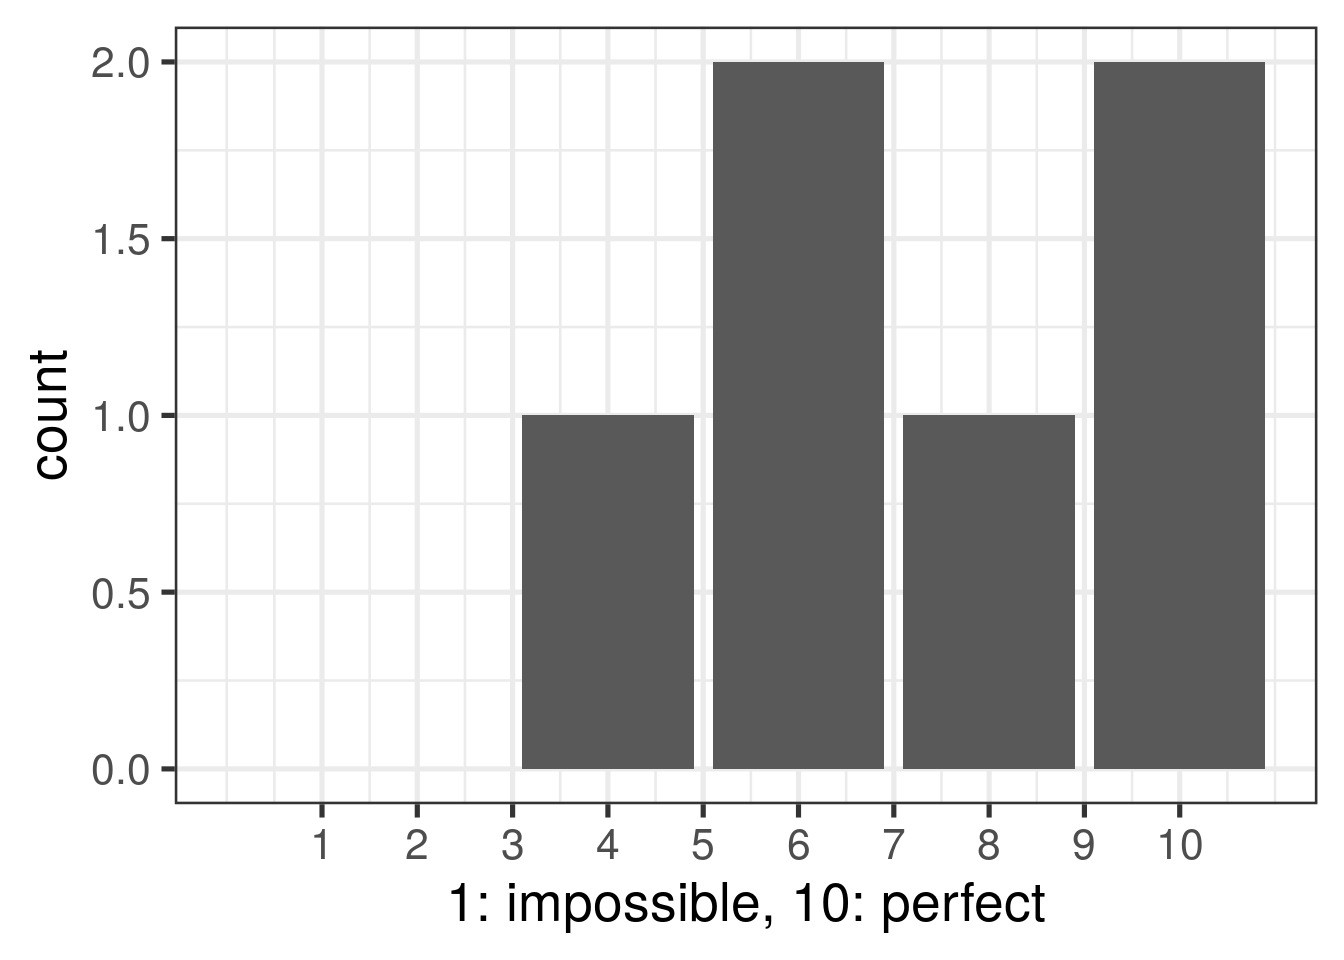
\includegraphics{_main_files/figure-latex/plot_48-1.pdf}

\hypertarget{how-often-do-you-encounter-issues-that-could-have-been-averted-if-things-were-better-organized-e.g.-missing-readme-or-github-repository.}{%
\section{How often do you encounter issues that could have been averted if things were better organized? E.g. missing README or GitHub repository.}\label{how-often-do-you-encounter-issues-that-could-have-been-averted-if-things-were-better-organized-e.g.-missing-readme-or-github-repository.}}

\begin{itemize}
\tightlist
\item
  Rarely
\item
  Monthly
\item
  Weekly
\item
  Weekly
\item
  Rarely
\item
  Weekly
\end{itemize}

\hypertarget{please-tell-me-more-about-the-kinds-of-organizational-issues-you-have-encountered-and-any-suggestions-to-improve-such-issues.}{%
\section{Please tell me more about the kinds of organizational issues you have encountered and any suggestions to improve such issues.}\label{please-tell-me-more-about-the-kinds-of-organizational-issues-you-have-encountered-and-any-suggestions-to-improve-such-issues.}}

\begin{itemize}
\tightlist
\item
  Others' code is often not documented, or context for performing certain code does not exist.
\item
  NA
\item
  Mostly just messy directories and filenames. I like the move to ``by-grant'' organization on JHPCE.
\item
  I have not encountered any issue
\item
  still need improvement on interactions with broader institute.
\item
  Sometimes I get handed scripts to use as examples and I have a hard time finding the data objects that the scripts are using. Or I have a hard time finding the output of the scripts.
\end{itemize}

\hypertarget{what-is-your-opinion-of-the-level-of-technical-support-in-the-team}{%
\section{What is your opinion of the level of technical support in the team?}\label{what-is-your-opinion-of-the-level-of-technical-support-in-the-team}}

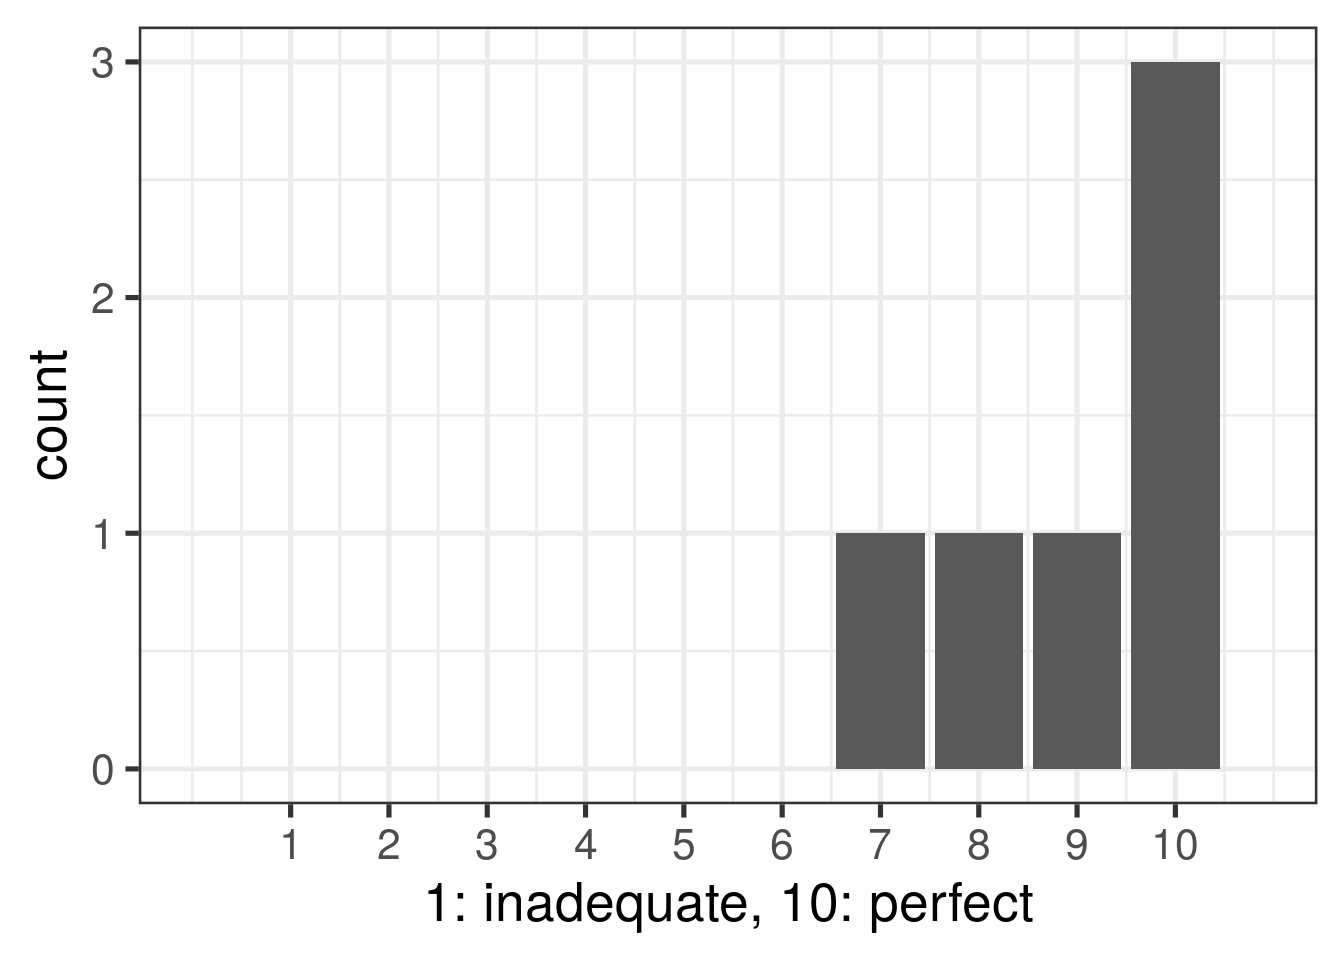
\includegraphics{_main_files/figure-latex/plot_51-1.pdf}

\hypertarget{what-is-your-opinion-of-the-level-of-administrative-support-in-the-team}{%
\section{What is your opinion of the level of administrative support in the team?}\label{what-is-your-opinion-of-the-level-of-administrative-support-in-the-team}}

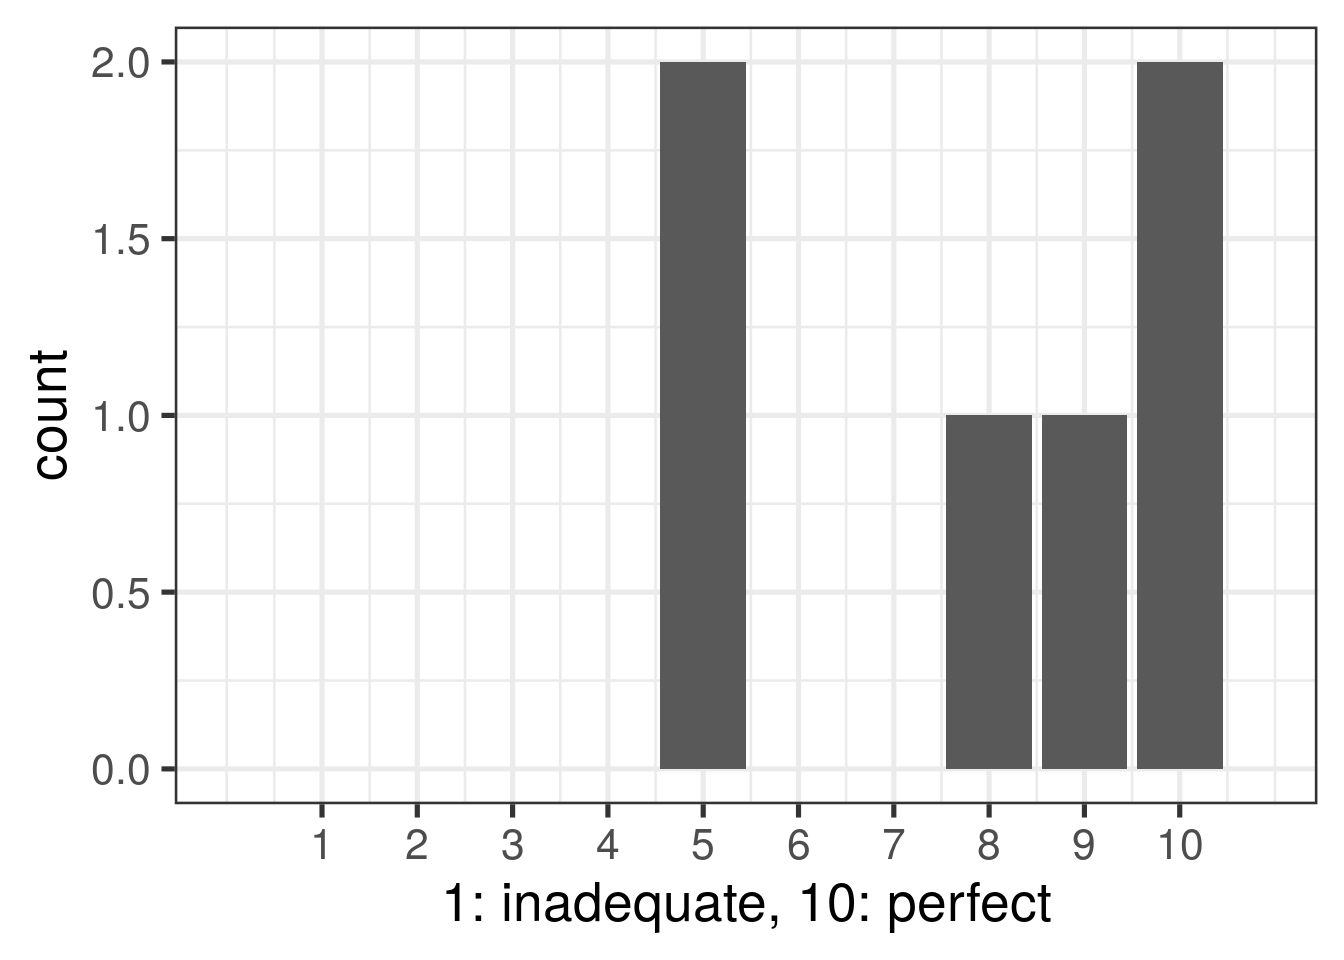
\includegraphics{_main_files/figure-latex/plot_52-1.pdf}

\hypertarget{what-is-your-impression-of-the-funding-of-the-team}{%
\section{What is your impression of the funding of the team?}\label{what-is-your-impression-of-the-funding-of-the-team}}

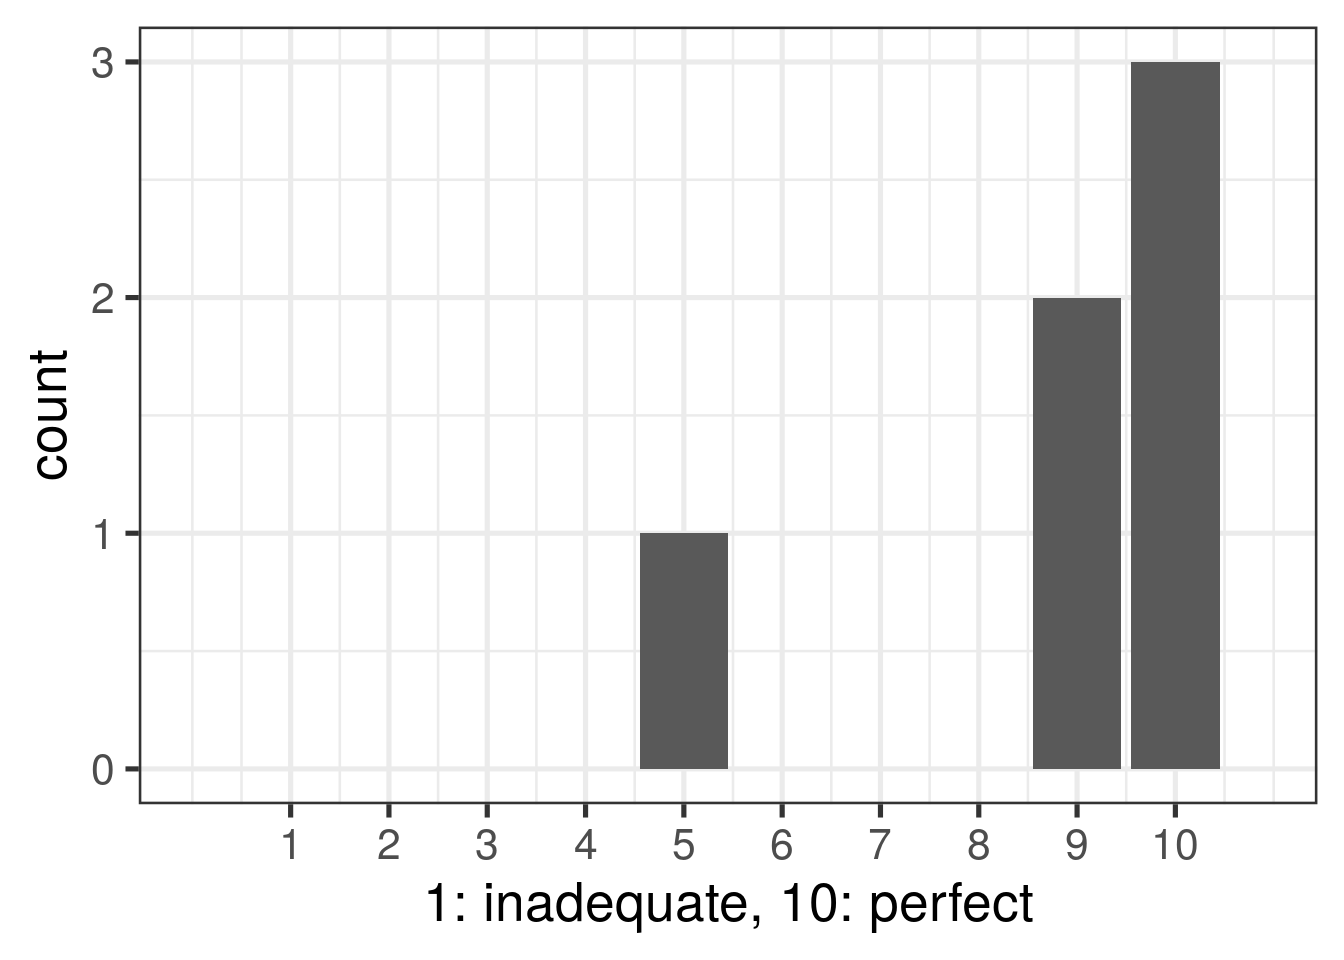
\includegraphics{_main_files/figure-latex/plot_53-1.pdf}

\hypertarget{if-we-had-the-funds-to-hire-one-more-full-time-person-what-kind-of-person-should-we-hire-and-what-role-would-they-play-in-the-team}{%
\section{If we had the funds to hire one more full-time person, what kind of person should we hire and what role would they play in the team?}\label{if-we-had-the-funds-to-hire-one-more-full-time-person-what-kind-of-person-should-we-hire-and-what-role-would-they-play-in-the-team}}

\begin{itemize}
\tightlist
\item
  I'm not sure about that
\item
  I'm not sure what is needed.
\item
  Staff scientist level/post-doc would be perfect
\item
  Someone who has strong R and or python skills and has studied/and experience in bioinformatics. As for role, more analysis work (idk this is a hard one to answer)
\item
  A math-y person to help explain the type of statistics we use.
\item
  I feel like someone to take some of the pressure off your load would be helpful to the team. You seem very busy and sometimes it would be nice to have someone with about your level of knowledge and experience (or even slightly less) to consult about certain issues.
\end{itemize}

\hypertarget{is-there-something-that-you-experienced-in-a-previous-job-that-you-wish-we-also-did-here}{%
\section{Is there something that you experienced in a previous job that you wish we also did here?}\label{is-there-something-that-you-experienced-in-a-previous-job-that-you-wish-we-also-did-here}}

\begin{itemize}
\tightlist
\item
  Raises
\item
  No.
\item
  NA
\item
  Absolutely not
\item
  No
\item
  Team meeting where people presented one slide (usually a graph) of what they did on their project that week
\end{itemize}

\hypertarget{are-there-any-concerns-or-other-areas-of-the-team-you-believe-could-be-improved-that-have-not-been-addressed-in-previous-questions-please-list-any-other-areas-you-think-could-be-improved-or-should-be-addressed.}{%
\section{Are there any concerns or other areas of the team you believe could be improved that have not been addressed in previous questions? Please list any other areas you think could be improved or should be addressed.}\label{are-there-any-concerns-or-other-areas-of-the-team-you-believe-could-be-improved-that-have-not-been-addressed-in-previous-questions-please-list-any-other-areas-you-think-could-be-improved-or-should-be-addressed.}}

\begin{itemize}
\tightlist
\item
  NA
\item
  My only concern at the institute is that sometimes the amount of information on slack can be overwhelming.
\item
  Returning to the lab expirations and timeline
\item
  No.
\item
  No
\item
  No
\end{itemize}

\hypertarget{finally-did-you-find-this-survey-useful-if-yes-how-often-should-the-survey-be-conducted}{%
\section{Finally, did you find this survey useful? If yes, how often should the survey be conducted?}\label{finally-did-you-find-this-survey-useful-if-yes-how-often-should-the-survey-be-conducted}}

\begin{itemize}
\tightlist
\item
  Yes, maybe every 6 months.
\item
  It was useful, but it was a bit long. I think yearly for something this long, maybe something more concise if we would do it with more frequency. Also in a group this small I feel like it is only so anonymous and we have a lot of discussions about this kind of stuff as a group already.\\
\item
  Somewhat. This could maybe be a yearly thing (or a couple times a year).
\item
  Yes
\item
  The survey is good and could be conducted annually. Some of the 1-10 questions could confuse people wo don't read the question well enough on their initial read (like me), because they use the 10-end of the scale to represent a lower magnitude of something bad (like `Not pressured') and the 1-end of the scale to represent a higher magnitude of something bad (like `Very pressured'). Ultimately not a problem for me because I re-read the scale labels but this might cause some erroneous answers.
\item
  Yes
\end{itemize}

\end{document}
